\documentclass[]{book}
\usepackage{lmodern}
\usepackage{amssymb,amsmath}
\usepackage{ifxetex,ifluatex}
\usepackage{fixltx2e} % provides \textsubscript
\ifnum 0\ifxetex 1\fi\ifluatex 1\fi=0 % if pdftex
  \usepackage[T1]{fontenc}
  \usepackage[utf8]{inputenc}
\else % if luatex or xelatex
  \ifxetex
    \usepackage{mathspec}
  \else
    \usepackage{fontspec}
  \fi
  \defaultfontfeatures{Ligatures=TeX,Scale=MatchLowercase}
\fi
% use upquote if available, for straight quotes in verbatim environments
\IfFileExists{upquote.sty}{\usepackage{upquote}}{}
% use microtype if available
\IfFileExists{microtype.sty}{%
\usepackage{microtype}
\UseMicrotypeSet[protrusion]{basicmath} % disable protrusion for tt fonts
}{}
\usepackage[margin=1in]{geometry}
\usepackage{hyperref}
\hypersetup{unicode=true,
            pdftitle={The Internetrix Advanced Guide to Attribution Modelling},
            pdfauthor={Dean Marchiori - Head of Data Science, Internetrix; Tiffany Chen - Data Analyst, Internetrix},
            pdfborder={0 0 0},
            breaklinks=true}
\urlstyle{same}  % don't use monospace font for urls
\usepackage{natbib}
\bibliographystyle{apalike}
\usepackage{color}
\usepackage{fancyvrb}
\newcommand{\VerbBar}{|}
\newcommand{\VERB}{\Verb[commandchars=\\\{\}]}
\DefineVerbatimEnvironment{Highlighting}{Verbatim}{commandchars=\\\{\}}
% Add ',fontsize=\small' for more characters per line
\usepackage{framed}
\definecolor{shadecolor}{RGB}{248,248,248}
\newenvironment{Shaded}{\begin{snugshade}}{\end{snugshade}}
\newcommand{\KeywordTok}[1]{\textcolor[rgb]{0.13,0.29,0.53}{\textbf{#1}}}
\newcommand{\DataTypeTok}[1]{\textcolor[rgb]{0.13,0.29,0.53}{#1}}
\newcommand{\DecValTok}[1]{\textcolor[rgb]{0.00,0.00,0.81}{#1}}
\newcommand{\BaseNTok}[1]{\textcolor[rgb]{0.00,0.00,0.81}{#1}}
\newcommand{\FloatTok}[1]{\textcolor[rgb]{0.00,0.00,0.81}{#1}}
\newcommand{\ConstantTok}[1]{\textcolor[rgb]{0.00,0.00,0.00}{#1}}
\newcommand{\CharTok}[1]{\textcolor[rgb]{0.31,0.60,0.02}{#1}}
\newcommand{\SpecialCharTok}[1]{\textcolor[rgb]{0.00,0.00,0.00}{#1}}
\newcommand{\StringTok}[1]{\textcolor[rgb]{0.31,0.60,0.02}{#1}}
\newcommand{\VerbatimStringTok}[1]{\textcolor[rgb]{0.31,0.60,0.02}{#1}}
\newcommand{\SpecialStringTok}[1]{\textcolor[rgb]{0.31,0.60,0.02}{#1}}
\newcommand{\ImportTok}[1]{#1}
\newcommand{\CommentTok}[1]{\textcolor[rgb]{0.56,0.35,0.01}{\textit{#1}}}
\newcommand{\DocumentationTok}[1]{\textcolor[rgb]{0.56,0.35,0.01}{\textbf{\textit{#1}}}}
\newcommand{\AnnotationTok}[1]{\textcolor[rgb]{0.56,0.35,0.01}{\textbf{\textit{#1}}}}
\newcommand{\CommentVarTok}[1]{\textcolor[rgb]{0.56,0.35,0.01}{\textbf{\textit{#1}}}}
\newcommand{\OtherTok}[1]{\textcolor[rgb]{0.56,0.35,0.01}{#1}}
\newcommand{\FunctionTok}[1]{\textcolor[rgb]{0.00,0.00,0.00}{#1}}
\newcommand{\VariableTok}[1]{\textcolor[rgb]{0.00,0.00,0.00}{#1}}
\newcommand{\ControlFlowTok}[1]{\textcolor[rgb]{0.13,0.29,0.53}{\textbf{#1}}}
\newcommand{\OperatorTok}[1]{\textcolor[rgb]{0.81,0.36,0.00}{\textbf{#1}}}
\newcommand{\BuiltInTok}[1]{#1}
\newcommand{\ExtensionTok}[1]{#1}
\newcommand{\PreprocessorTok}[1]{\textcolor[rgb]{0.56,0.35,0.01}{\textit{#1}}}
\newcommand{\AttributeTok}[1]{\textcolor[rgb]{0.77,0.63,0.00}{#1}}
\newcommand{\RegionMarkerTok}[1]{#1}
\newcommand{\InformationTok}[1]{\textcolor[rgb]{0.56,0.35,0.01}{\textbf{\textit{#1}}}}
\newcommand{\WarningTok}[1]{\textcolor[rgb]{0.56,0.35,0.01}{\textbf{\textit{#1}}}}
\newcommand{\AlertTok}[1]{\textcolor[rgb]{0.94,0.16,0.16}{#1}}
\newcommand{\ErrorTok}[1]{\textcolor[rgb]{0.64,0.00,0.00}{\textbf{#1}}}
\newcommand{\NormalTok}[1]{#1}
\usepackage{longtable,booktabs}
\usepackage{graphicx,grffile}
\makeatletter
\def\maxwidth{\ifdim\Gin@nat@width>\linewidth\linewidth\else\Gin@nat@width\fi}
\def\maxheight{\ifdim\Gin@nat@height>\textheight\textheight\else\Gin@nat@height\fi}
\makeatother
% Scale images if necessary, so that they will not overflow the page
% margins by default, and it is still possible to overwrite the defaults
% using explicit options in \includegraphics[width, height, ...]{}
\setkeys{Gin}{width=\maxwidth,height=\maxheight,keepaspectratio}
\IfFileExists{parskip.sty}{%
\usepackage{parskip}
}{% else
\setlength{\parindent}{0pt}
\setlength{\parskip}{6pt plus 2pt minus 1pt}
}
\setlength{\emergencystretch}{3em}  % prevent overfull lines
\providecommand{\tightlist}{%
  \setlength{\itemsep}{0pt}\setlength{\parskip}{0pt}}
\setcounter{secnumdepth}{5}
% Redefines (sub)paragraphs to behave more like sections
\ifx\paragraph\undefined\else
\let\oldparagraph\paragraph
\renewcommand{\paragraph}[1]{\oldparagraph{#1}\mbox{}}
\fi
\ifx\subparagraph\undefined\else
\let\oldsubparagraph\subparagraph
\renewcommand{\subparagraph}[1]{\oldsubparagraph{#1}\mbox{}}
\fi

%%% Use protect on footnotes to avoid problems with footnotes in titles
\let\rmarkdownfootnote\footnote%
\def\footnote{\protect\rmarkdownfootnote}

%%% Change title format to be more compact
\usepackage{titling}

% Create subtitle command for use in maketitle
\newcommand{\subtitle}[1]{
  \posttitle{
    \begin{center}\large#1\end{center}
    }
}

\setlength{\droptitle}{-2em}

  \title{The Internetrix Advanced Guide to Attribution Modelling}
    \pretitle{\vspace{\droptitle}\centering\huge}
  \posttitle{\par}
  \subtitle{With applications in R}
  \author{Dean Marchiori - Head of Data Science, Internetrix \\ Tiffany Chen - Data Analyst, Internetrix}
    \preauthor{\centering\large\emph}
  \postauthor{\par}
      \predate{\centering\large\emph}
  \postdate{\par}
    \date{2019-05-07}

\usepackage{booktabs}
\usepackage{amsthm}
\makeatletter
\def\thm@space@setup{%
  \thm@preskip=8pt plus 2pt minus 4pt
  \thm@postskip=\thm@preskip
}
\makeatother  
\let\oldmaketitle\maketitle
\AtBeginDocument{\let\maketitle\relax}

\begin{document}
\maketitle

\thispagestyle{empty}
\begin{center}

\includegraphics{cover.png}
\end{center}

\let\maketitle\oldmaketitle
\maketitle

{
\setcounter{tocdepth}{1}
\tableofcontents
}
\chapter{Welcome}\label{welcome}

The aim of this guide is to help marketing, business and analytics
experts understand how to get the biggest impact from their marketing
budget.

Our focus is on marketing attribution. That is, the way in which we can
measure and assign credit to individual marketing channels, even when we
are simultaneously advertising via many channels. Only by understanding
this can we generate meaningful estimates on the return we get from each
channel and therefore guide future spending decisions.

When we say marketing, the main focus is on digital marketing. In this
guide we use Google Analytics and the Google Marketing Platform as the
tools of choice. If you use some other digital analytics platform, you
can still benefit from the content, but you will need to be a little
more self-sufficient in exporting and preparing your data for analysis.

Finally, for more advanced and customised methods we use the R
statistical programming language. These sections are aimed at data
scientists and data analysts with some experience with scripted
analysis. Hopefully the basic examples shown in this guide will help in
getting up to speed and generating useful insights as quickly as
possible.

We hope you enjoy and get some benefit from this guide. If you have any
feedback or comments, or would like to discuss working together, please
reach out using the contact information below.

\section{Contact Internetrix}\label{contact-internetrix}

\textbf{Internetrix Data Science}

\textbf{Web:}
\url{https://www.internetrix.com.au/services/data-science/}\\
\textbf{Phone:} +61242535300\\
\textbf{email:}
\href{mailto:irx.info@internetrix.com.au}{\nolinkurl{irx.info@internetrix.com.au}}

This work is licensed under a Creative Commons
Attribution-NonCommercial-NoDerivatives 4.0 International License.

\chapter{Introduction}\label{introduction}

\section{What is attribution
modelling}\label{what-is-attribution-modelling}

The ideal world for marketers is that customers will fall in love with
your products or services and make a purchase the first time they see an
advertisement. But, the truth is the customer might have hundreds of
interactions with a brand before they make a purchase. Actually, they
might get exposed to the products or services through different
marketing channels such as social media, other web sites, search engines
and apps etc.

So why do we care about this? The ultimate aim is to arm decision makers
with the data needed to make complex decisions. We do this by measuring
the return on investment (ROI) of marketing efforts. In Jayawardane et.
al (2015) they discuss how customers who interact with a brand across
multiple channels bring in more value. While it is typical to have
parallel streams of marketing efforts, it is not straightforward to
understand which of these channels actually helped make the conversion
and to what extent.

We present a tour of methods that solve this problem with practical
implementation guides and code examples. We aim to give decision makers
the data to understand the true return from each channel and therefore
guide marketing strategy in a data driven way.

\section{Definitions}\label{definitions}

In this guide we talk about the `customer pathway' or the `conversion
journey'. We define this as the sequence of steps a customer takes when
interacting with a brand which will ultimately lead to either the
customer converting or not converting.

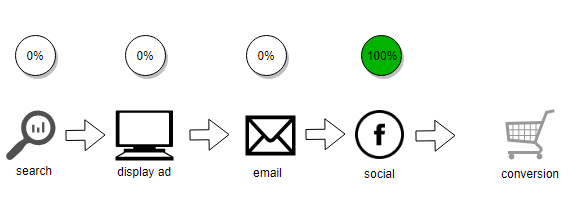
\includegraphics[width=5.88in]{img/last_touch}

We say \emph{conversion} to mean the user has completed a desired
action. This may indeed be purchasing an item from a website eStore,
however in other domains this may simply mean signing up to a service or
newsletter or completing some other pre-defined action.

\section{Scope of this paper}\label{scope-of-this-paper}

First we break down the types of models that solve this attribution
problem in different ways.

For each type of approach we present an explanation and a practical
example of how they work as well as a review of their strengths and
weaknesses.

At Internetrix, we are accredited Google Partners and support clients
with tracking and optimising their online presence using tools from the
Google Marketing Platform. We review the existing methods that are
available in tools like Google Analytics and Analytics 360.

However, this guide is largely aimed at users who want to customise and
extend these methods and tailor them to their specific company goals. We
present a toolkit using the R programming language, complete with
reproducible code examples to showcase attribution modelling methods,
from the very basic to more complicated and powerful algorithms.

In doing this, we use example data from Google Analytics 360 and
BigQuery. We cover the often neglected steps of how to query and prepare
this data for modelling. However, for users who collect their digital
marketing data in other platforms, the implementation guides will still
be relevant and valuable.

Finally we extend attribution modelling in a bonus section to cover
\emph{offline} attribution. That is, measuring the impact of channels
outside the digital sphere like TV, radio, billboard etc. This unlocks
some powerful tools to extend beyond what is tracked from your website.

\section{Where to go for further
help}\label{where-to-go-for-further-help}

While not a complete guide, we hope it provides some insights to the
various methods that can help arm your organisation with the data to
make effective marketing decisions.

For further help please reach out to us any time:

\textbf{Internetrix Data Science}

\textbf{Web:}
\url{https://www.internetrix.com.au/services/data-science/}\\
\textbf{Phone:} +61242535300\\
\textbf{email:}
\href{mailto:irx.info@internetrix.com.au}{\nolinkurl{irx.info@internetrix.com.au}}

\part{Online Attribution}\label{part-online-attribution}

\chapter{Types of Attribution}\label{types-of-attribution}

\section{Group vs.~Individual
Attribution}\label{group-vs.individual-attribution}

Historically, marketers got inspired by the marketing performance and
strategies of offline channels such as newspaper and broadcasts, but
there were some drawbacks. For example, they could not be used for
investigating customer conversions at an \emph{individual} level.

Marketing attribution in this case was largely done at the group level
by aggregating the performance of all users responding via a particular
channel. Furthermore it was difficult and often impossible to understand
which customers experienced multiple touch points in these offline
channels.

Currently, the prevalence of digital marketing provides the marketer
with a better way to gain insights on how marketing activities perform
at the individual level.

\section{Simplistic vs.~Fractional
Modelling}\label{simplistic-vs.fractional-modelling}

\subsection{Simplistic modelling}\label{simplistic-modelling}

Simplistic models assign complete conversion credit to just a single
touch point. A consequence of this is all other touch points in a user's
conversion pathway are effectively ignored.

There are several types of simplistic attribution models, but we mainly
focus on two of them, which have been widely adopted. In the
\textbf{Last Touch} model, 100\% credit for a conversion is assigned to
the final touch point which happens before the conversion. In contrast,
in the \textbf{First Touch} model, 100\% credit is assigned to the first
touch point a customer uses in their conversion pathway.

\subsection{Fractional modelling}\label{fractional-modelling}

Unlike simplistic modelling techniques, fractional modelling determines
the `fractional' contribution of each touch point and helps the marketer
apply appropriate weights to all channels in a client's decision-making
journey.

Fractional attribution modelling is subdivided into heuristic modelling
and algorithmic modelling as discussed in more detail below.

\section{Heuristic vs.~Algorithmic
Modelling}\label{heuristic-vs.algorithmic-modelling}

\subsection{The Heuristic model}\label{the-heuristic-model}

The concept of the heuristic model, also known as rule-based fractional
modelling, is summarised in Jayawardane et. al (2015) who define it as
fixed rules to assign the credits to all touch points leading to the
conversion.

These `rules' that the heuristic modelling is based on include
\textbf{Linear}, \textbf{Position Based}, \textbf{Time Decay} and others
which we will explore further in later sections.

Compared to simplistic modelling, heuristic models better capture the
contributions of multiple advertising and marketing channels.

\subsection{The Algorithmic model}\label{the-algorithmic-model}

Extending the idea of fractional attribution is algorithmic attribution.

Rather than using a rule-of-thumb, an algorithmic model will analyse
both converting and non-converting paths customers take and make a
probabilistic assessment of each channel's contribution to a conversion.
Often using advanced statistics and machine learning algorithms,
algorithmic methods develop custom weightings for each channel based on
their effectiveness.

Currently, some popular approaches are Markov Chain models, the Shapley
Value and survival analysis. We will take a detailed look into these
methods and which are appropriate for your analysis goals.

\section{Classification of Methods}\label{classification-of-methods}

Below is a useful taxonomy of the commonly used methods for marketing
attribution modelling in eCommerce.

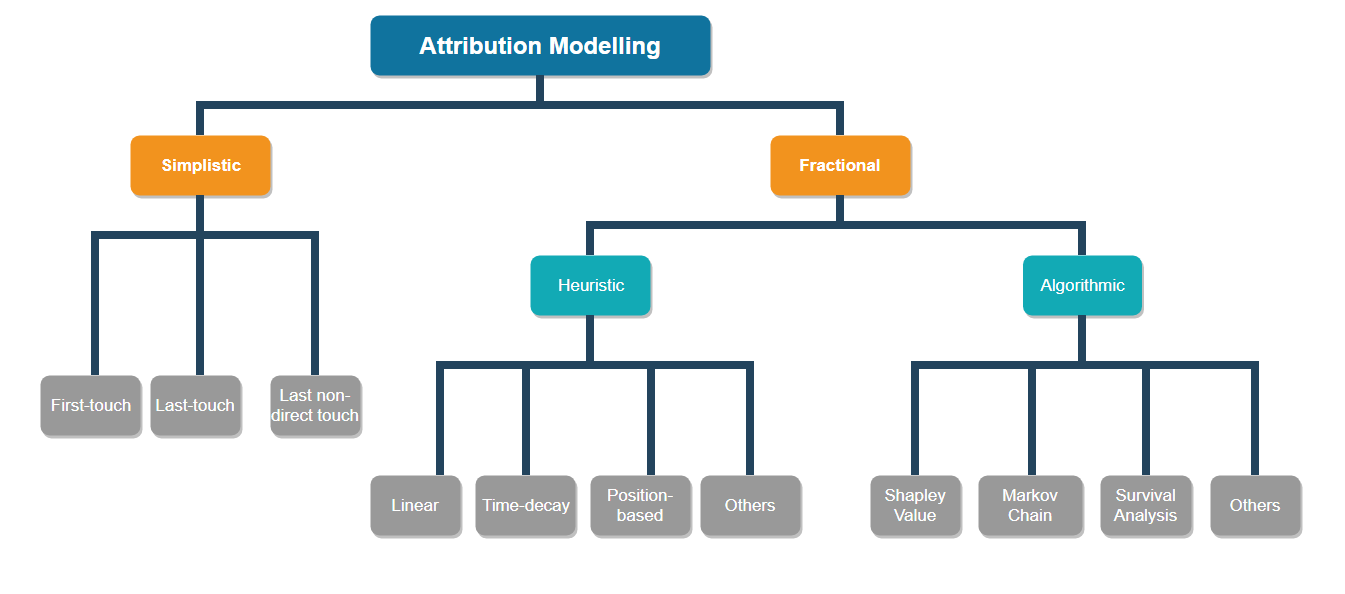
\includegraphics[width=6.72in]{img/attributionModel}

\chapter{Methods}\label{methods}

We will now take a practical tour of some common models for marketing
attribution.

\emph{A customer wants to buy some swimwear on your website. They start
with a Google search that leads them to your website, but no purchase is
made. A few days later they click on a display ad and go back to your
website, perhaps to take another look at the product range and sign up
for special offers. One week later they get an email campaign while at
work and click though to check for special deals, but don't yet
purchase. Later that evening, they see a Facebook ad and remember to
grab their credit card and make a purchase.}

So which channel caused this purchase? Was is the social channel that
drove the customer to purchase, or was it the search result that made
the customer initially aware of your brand, or was it the display and
email campaigns that re-engaged the customer?

We will now look at a few different methods for making this decision.

\section{Simplisitic Methods}\label{simplisitic-methods}

Simplistic methods assign credit for a conversion to just one
pre-determined touch point in the marketing journey. This is common and
robust, but quite naive way to assess your marketing performance.

\subsection{Last Touch}\label{last-touch}

A classic example of a simplistic method is \textbf{Last Touch}
attribution (sometimes also referred to as Last Interaction or Last
Click).

In this model, all credit for the sale is attributed to the very last
touch point in the customer's conversion pathway. In this case the
social channel.

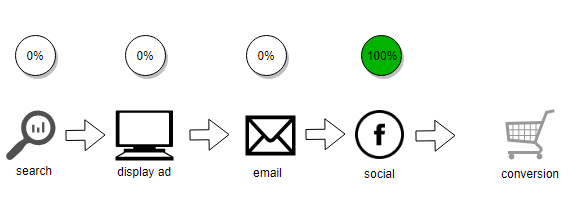
\includegraphics[width=5.88in]{img/last_touch}

\subsection{First Touch}\label{first-touch}

A \textbf{First Touch} model assigns all credit for a sale to the first
channel in a customer's conversion pathway. Here it is the search
channel.

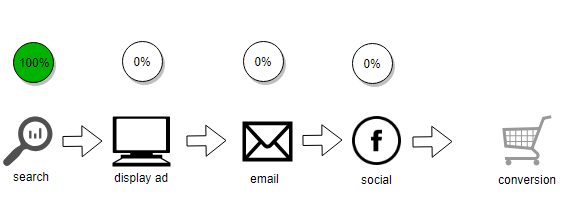
\includegraphics[width=5.65in]{img/first_touch}

\subsection{Others}\label{others}

There are a number of modifications to these that enable greater
refinement. For example \textbf{Last non-direct click} is the same as
Last Touch, but if the last touch is the direct channel, it ignores this
and looks back to the last pure marketing channel.

\section{Fractional Heuristic
Methods}\label{fractional-heuristic-methods}

In some specialised cases, a simplistic model may work well, however an
intuitive next step is to split the credit across all or several
channels that lead to the conversion. Just like a game of football, one
person scores the goal, but its the entire team that works together to
create the scoring opportunity.

\subsection{Linear}\label{linear}

The least opinionated method is known as the \textbf{Linear attribution
model}. This method assigns equal credit across all marketing channels
in the customer's conversion pathway.

In the example below all four touch points are assigned 25\% credit for
the value of the conversion.

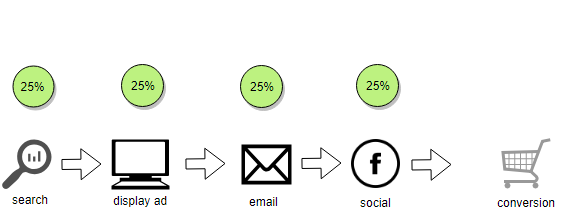
\includegraphics[width=5.61in]{img/linear}

\subsection{Time Decay}\label{time-decay}

In our scenario, considerable time passed between the first search,
looking at the display ad, then getting an email campaign. A natural
question is whether touch points from days or weeks ago really
contribute equally to touch points made the day of a purchase? A model
that accounts for this is the \textbf{Time Decay model}. This method
adjusts the credit given to each channel based on how long ago the touch
point occurred. This assigns less credit to distant touch points and
more weighting to recent activity.

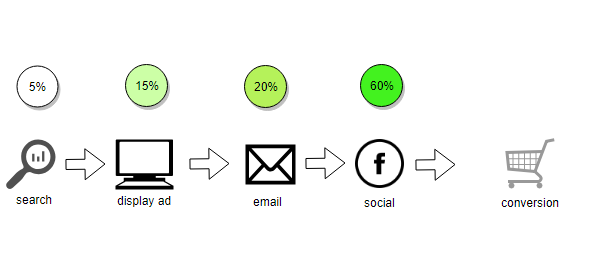
\includegraphics[width=5.92in]{img/time_decay}

\subsection{Position Based}\label{position-based}

Taking the concept of First Touch and Last Touch a step further, we can
arbitrarily define attribution rules based on where in the conversion
pathway a channel sits.

This is known as \textbf{Position Based} attribution. For example, below
we have assigned 45\% of the conversion credit to the first and last
touch points, with equal amounts allocated to all touch points in
between.

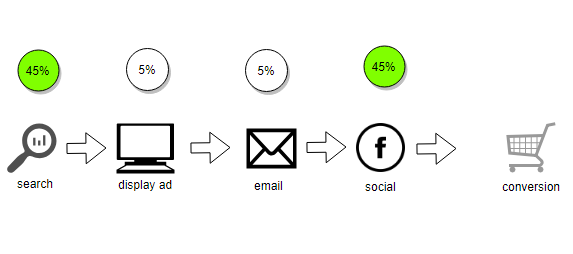
\includegraphics[width=5.73in]{img/position_based}

\section{Fractional Algorithmic
Methods}\label{fractional-algorithmic-methods}

Algorithmic attribution models attempt to use historical data on actual
conversion performance to measure or infer attribution, rather than rely
on human defined rules and heuristics.

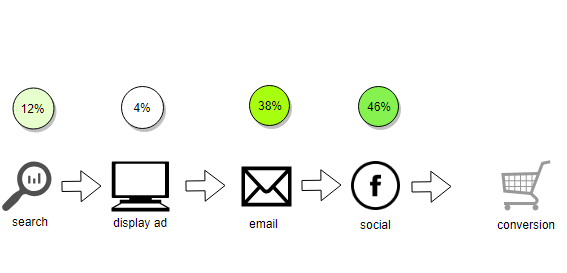
\includegraphics[width=5.67in]{img/fractional}

This is achieved through advanced statistical methods and algorithms
that account for individual channel performance. Often these methods
look at both the pathways for customers who converted and those who did
not. This is a step up in sophistication and objectivity that can add
tremendous value when simple rules are too naive to enable effective
decision making.

\subsection{Logistic Regression}\label{logistic-regression}

Logistic regression is a commonly used statistical procedure developed
in the 19th Century \citep{cramer2002origins}. In simple terms, it uses
a function known as the logistic function, to model a binary outcome.
This may be yes/no, true/false or in our case converted/not converted.
It bases this on a set of independent variables that may have
contributed to the outcome of choice.

As a fractional or multi-touch method, in our case this means
determining which marketing channels contributed to whether a customer
converted or not. Typically this means using the various marketing
channels (email, display, search) as covariates in the model. For each
customer journey, an indication will be made against each channel based
on whether or not it was part of the customers conversion journey. This
provides the basis for modelling the outcome of whether the customer
converted or not.

\begin{longtable}[]{@{}lllll@{}}
\toprule
customer & email & display & search & converted?\tabularnewline
\midrule
\endhead
12345 & TRUE & TRUE & FALSE & Yes\tabularnewline
38546 & FALSE & FALSE & TRUE & No\tabularnewline
48379 & TRUE & FALSE & FALSE & Yes\tabularnewline
\ldots{} & \ldots{} & \ldots{} & \ldots{} & \ldots{}\tabularnewline
\bottomrule
\end{longtable}

In practice, many of the channels will be related and gaining
statistically rigorous estimates can be challenging. Other statistical
techniques like `bagging' have been used to improve accuracy with these
methods \citep{shao2011data}.

\hypertarget{shapley-value}{\subsection{Shapley
Value}\label{shapley-value}}

The Shapley Value \citep{shapley1953value} originated in 1953 by Nobel
Prize winning mathematician Lloyd Shapley. It is a concept in Game
Theory, specifically in systems where many factors need to cooperate to
achieve a given outcome. The Shapley Value is a way of allocating credit
for the total outcome achieved amongst these many cooperating factors.

In terms of a marketing example, we can see a comparison of two pathways
below. Including `Display' in the sequence increases the likelihood of a
purchase by 2\%. Therefore we can attribute this increase to `Display'
despite it being only a link in the sequence. To get the complete credit
given to Display, more historical comparisons need to be made with
Display occurring at different locations and working with different
touch points.

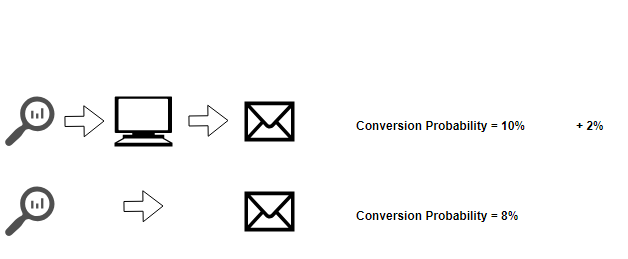
\includegraphics[width=6.28in]{img/shapley}

For the technically inclined, the formula to calculate the Shapley value
for a given contributor is:

\[
\phi_i(v) = \frac{1}{\mid{N!}\mid}\sum_{R}[v(P_i^R \cup \{i\}) - v(P_i^R)]
\]

To translate this, for any given marketing touch point (e.g.~Display),
what is the pay-off achieved where Display is part of the pathway
sequence. Subtract from this the marginal contributions made by all the
touch points preceding it. Add these contributions up across all
permutations containing Display and divide by the total number of
possible pathway permutations. This gives us our weighted marginal
contribution to the overall outcome for a given marketing channel.

\hypertarget{markov-methods}{\subsection{Markov
Methods}\label{markov-methods}}

A Markov Chain is a mathematical system that models events that
transition from one `state' to another. These states could be a touch
point in a marketing journey, the current day's weather or the health
status of a patient. These concepts are explored further in
\citep{gagniuc2017markov}.

By recording the probability of moving from one state to another a
prediction of future states can be made by knowing the present state of
the system.

A Markov Chain is defined by three properties:

\begin{itemize}
\tightlist
\item
  The state space -- the set of all the states in which process could
  potentially exist
\item
  The transition matrix -- the probability of moving from one state to
  other state
\item
  current state probability distribution -- probability distribution of
  being in any one of the states at the start of the process.
\end{itemize}

Markov chains are stochastic processes, but they have a characteristic
of being `memory-less'. This means the predictions they make depend only
on the present state of the system. Having said that, an extension to
discrete time markov chains is the ability to use different `order'
models to account for a small number of previous states when making
future predictions. We will explore this further in
\protect\hyperlink{markov-chains}{Section 9.1}.

A basic way to think about markov chains is via weather. If we look at
some historical data on whether it is sunny, cloudy or rainy we can form
probabilities of moving from one of these states to another. Intuitively
if it's sunny today, we could reasonably expect a high likelihood of
sunny weather tomorrow. Conversely, if it is raining today then cloud or
rain are probably more likely than sunshine tomorrow.

We can view these probabilities as a `transition matrix', and even plot
them as a directed network graph.

\begin{tabular}{l|r|r|r}
\hline
  & sunny & cloudy & rain\\
\hline
sunny & 0.7 & 0.20 & 0.10\\
\hline
cloudy & 0.3 & 0.40 & 0.30\\
\hline
rain & 0.2 & 0.45 & 0.35\\
\hline
\end{tabular}

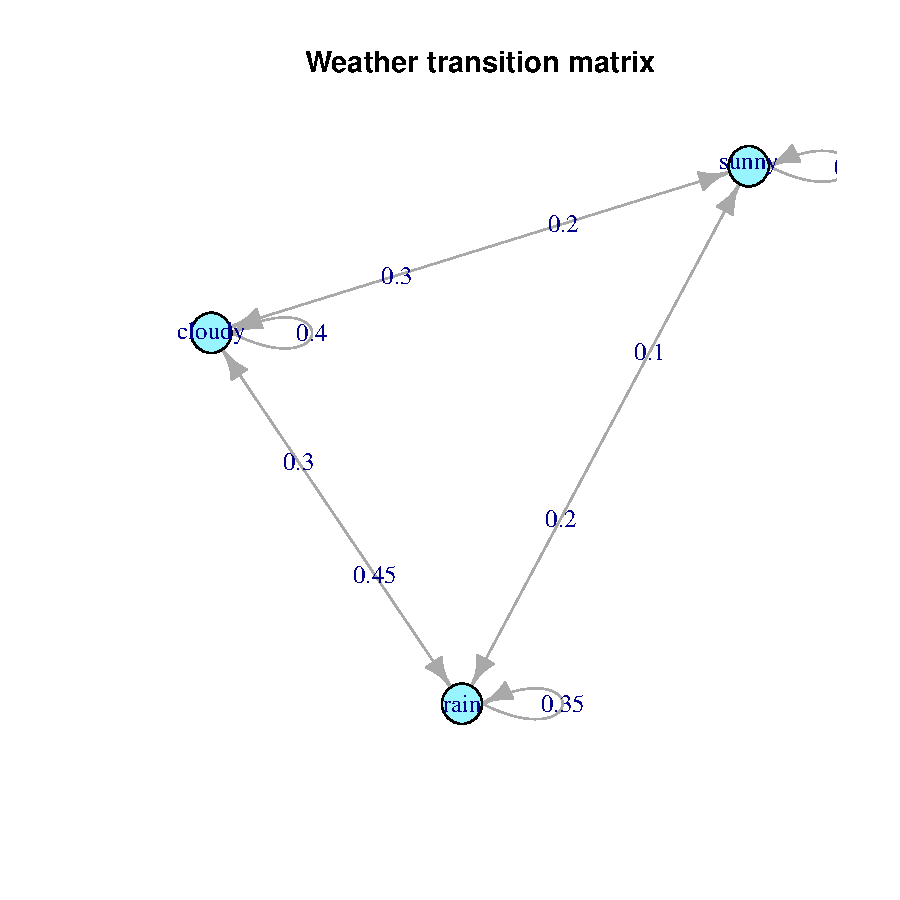
\includegraphics{irx-attribution-2019_files/figure-latex/unnamed-chunk-16-1.pdf}

If we know it is cloudy today we can represent that as:

\[
initial = \begin{bmatrix} sunny = 0 \\ cloudy = 1 \\ rain = 0\end{bmatrix}
\]

By multiplying this into the transition matrix, we can get the
probabilities of the the weather tomorrow. We can also simply read this
result off our initial transition matrix.

\begin{tabular}{r|r|r}
\hline
sunny & cloudy & rain\\
\hline
0.3 & 0.4 & 0.3\\
\hline
\end{tabular}

We can continue this multiplication several times to forecast ahead say,
seven days:

\begin{tabular}{r|r|r}
\hline
sunny & cloudy & rain\\
\hline
0.4622776 & 0.3188612 & 0.2188612\\
\hline
\end{tabular}

So how does this relate to marketing attribution? If we define the
states in our model to be the various touch points, such as
\texttt{email}, \texttt{paid\ search}, \texttt{display},
\texttt{social}, and include states such as \texttt{start},
\texttt{end}, \texttt{converted} we can fully articulate our multi touch
attribution model by observing the historical probability of customers
moving from one state to another.

Once we have this graph defined we can measure the importance of each
touch point by removing them one-by-one and simulating the resulting
impact on conversions. This is known as the `Removal Effect'
\citep{removal2018} and is covered in more detail in the practical
section in \protect\hyperlink{markov-chains}{Section 9.1}. It is a
simple way to extend our ideas of multi-touch attribution beyond basic
rule based methods.

\subsection{Survivial Analysis}\label{survivial-analysis}

Survival analysis is a type of statistical analysis to model
`time-to-event' data. The name `survival' evokes a medical application
such as modelling how long diseased patients may survive under various
treatments, however the method is applicable across a wide range of
domains.

The key components of a survival analysis are
\citep{noauthor_survival_2019}:

\begin{itemize}
\tightlist
\item
  \textbf{Event}: This is the thing of interest, it may be death,
  machine failure, or sales conversion etc.\\
\item
  \textbf{Time}: The time from the beginning of an analysis period to
  either the end of the study period or until the event of interest
  occurs, or disqualification from the analysis.\\
\item
  \textbf{Censoring}: A key feature of survival analysis is censoring,
  which flags which observations did not experience the event in the
  time period of the analysis.\\
\item
  \textbf{Survival Function}: The probability that a subject survives
  longer than time t.
\end{itemize}

The concept of censoring is a clear distinction with this method. While
a customer may be exposed to a marketing campaign, if they do not
convert in the time period of the analysis, we cannot conclude they wont
ever convert, just we have not observed a conversion event in our
analysis time period.

A common method for estimating a survival function is with the use of a
Kaplan-Meier curve \citep{kaplan1958nonparametric} which can be used to
display a chart of declining horizontal steps over time, which
approximates the true survival function.

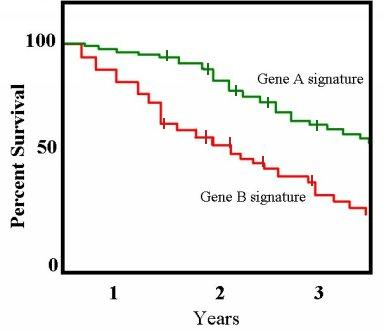
\includegraphics[width=3.84in]{img/Km_plot} source:
\url{https://upload.wikimedia.org/wikipedia/commons/7/73/Km_plot.jpg}

Mathematically this can be defined as

\[
\hat{S}(t) = \prod\limits_{i: t_i \leq{t}} (1 - \frac{d_i}{n_i})
\]

Where \(\hat{S(t)}\) is our estimator of survival (non-conversion) at
time \(t\). This formula looks at small time periods where events occur
and calculates the survival probability based on the number of subjects
who are still around at that time period.

There are many ways to extend this idea to marketing attribution. Rather
than looking at assigning credit to touch points, we will take a
slightly different approach.

In the practical section in
\protect\hyperlink{survival-analysis}{section 9.2} we will compute an
estimate for the survival function and stratify this by the channel in
which our users converted. By doing this we can understand the
likelihood of conversion though different channels at varying times
throughout a typical conversion journey. This adds an interesting new
dimension to analysing marketing performance.

\section{Comparison of Methods}\label{comparison-of-methods}

So which model is the right one to use? There is no clear cut answer. A
one-size-fits-all model to attributing marketing credit does not exist
\citep{shao2011data}.

The choice should be determined by an understanding of the goals of your
marketing activities and how they drive business outcomes. As a general
rule, without substantive justification, heuristic and simplistic
methods are very subjective and should only serve as a baseline over the
data-driven methods.

\chapter{Google Analytics Data}\label{google-analytics-data}

Google Analytics users can benefit from a range of simple and heuristic
attribution models for their digital data, build right into the
platform. \citep{noauthor_google_nodate}

This is a great start, but they have one thing in common - they are
heuristics. In other words, you ultimately make the decision on which
model to use and this logic is hard-wired into the report. While these
methods are quite intuitive, they are also quite naive.

\section{Survey of Basic Methods in Google
Analytics}\label{survey-of-basic-methods-in-google-analytics}

\begin{itemize}
\tightlist
\item
  \textbf{Last Interaction}
\item
  \textbf{First Interaction}
\item
  \textbf{Linear}
\item
  \textbf{Time Decay}
\item
  \textbf{Last Non-Direct Click}
\item
  \textbf{Last Google Ads Click}
\item
  \textbf{Position Based}
\end{itemize}

A full overview is contained on the
\href{https://support.google.com/analytics/answer/1665189?hl=en\&ref_topic=3205717}{Google
Help Pages}

Google also has a useful feature called the
\href{https://support.google.com/analytics/answer/6148697}{Model
Comparison Tool} which allows the comparison of up to 3 attribution
models at once.

\section{About Data Driven
Attribution}\label{about-data-driven-attribution}

Google's
\href{https://support.google.com/analytics/answer/3264076?\%20hl=en\&ref_topic=3180362}{Data-Driven
Attribution} is a feature only available in Google Analytics 360, part
of Google Marketing Platform. Rather than using the position-based
heuristics above, Data-Driven Attribution uses real data from your
Google Analytics account to generate a custom model, driven by a more
sophisticated algorithm.

\subsection{How does it work?}\label{how-does-it-work}

The more basic, position-based methods are only interested in the paths
that led to a conversion. Google's Data-Driven Attribution model
analyses both converting and non-converting pathways. According to
Google, it has two main steps:

\begin{enumerate}
\def\labelenumi{\arabic{enumi}.}
\item
  Analyse all available path data to develop a probabilistic model of
  how customer journey's progress on your site.
\item
  Apply a sophisticated algorithm to this data to assign credit to
  particular marketing touch points.
\end{enumerate}

The algorithm used in Data-Driven Attribution is based on a concept
called the Shapley Value \protect\hyperlink{shapley-value}{See Section
4.3.2}, which is from the field of cooperative game theory. This method
recognises the contribution a marketing touch point makes depends on
where in the conversion pathway it occurs. By comparing many similar
customer pathway sequences both with and without a given touch point
included, a form of weighted contribution can be calculated. Put another
way, intuitively this is like removing a particular marketing channel
from a sequence of touch points in a user's journey and wondering what
downstream impact it would have on conversions.

\subsection{Limitations}\label{limitations}

There are some important factors to be aware of with Data-Driven
Attribution. Firstly, the results presented are refreshed by Google on a
weekly basis and look back at the last 28 days of conversion history at
the time the model is trained. The benefit here is that models will
evolve as your online activity does. Also, the model will only look back
to a maximum of 4 interactions within the prior 90 days to each
conversion.

Given this method learns from historical data, for the results to be
meaningful there are thresholds imposed. These thresholds set the
minimum amount of pathways and conversions to ensure there is enough
data to train the model. At the time of writing these thresholds are:

\begin{itemize}
\tightlist
\item
  400 conversions per conversion type with a path length of 2+
  interactions (i.e., 400 conversions for a specific goal or
  transaction, not a sum of 400 over all conversion types) AND\\
\item
  10,000 paths in the selected reporting view (roughly equivalent to
  10,000 users, although a single user may generate multiple paths)
\end{itemize}

\section{BigQuery}\label{bigquery}

\begin{quote}
BigQuery is a Google Developers tool that lets you run super-fast
queries of large datasets.
\end{quote}

While Google Analytics contains a plethora of online tool for analysis,
when aiming to conduct more advanced digital analytics and attribution
modelling, having \emph{all} of your hit level data available is key.
\citep{noauthor_bigquery_nodate}

For customers that use Google Analytics 360 as part of the Google
Marketing Platform, they have access to the
\href{https://support.google.com/analytics/answer/3437618?hl=en\&ref_topic=3416089}{BigQuery
Export for Analytics.}

Using BigQuery lets you access both session and hit level data using an
SQL like syntax. Plus you benefit from the speed and scale of BigQuery
along with the ability to create tables, data sets and manage jobs with
your data.

\part{Implementation
Guides}\label{part-implementation-guides}

\chapter{Setup}\label{setup}

Before we start with the practical guides, it is important to ensure we
correctly install and setup the required dependencies.

\section{R}\label{r}

\subsection{About R}\label{about-r}

The R programming language \citep{R-base} is a popular and open-source
tool for data analysis and statistical computing.

We will use R throughout this paper for the practical examples.


\includegraphics[width=1in]{img/R}

\subsection{Install R}\label{install-r}

To install R, head over to \url{https://www.r-project.org/} and follow
the instructions.

It will prompt you to choose a CRAN Mirror. This is an archive server
that contains the latest R version.

There are instructions to install R on Linux, Mac and Windows.

This will install the base R software, which on its own is just a
command line-like interface.

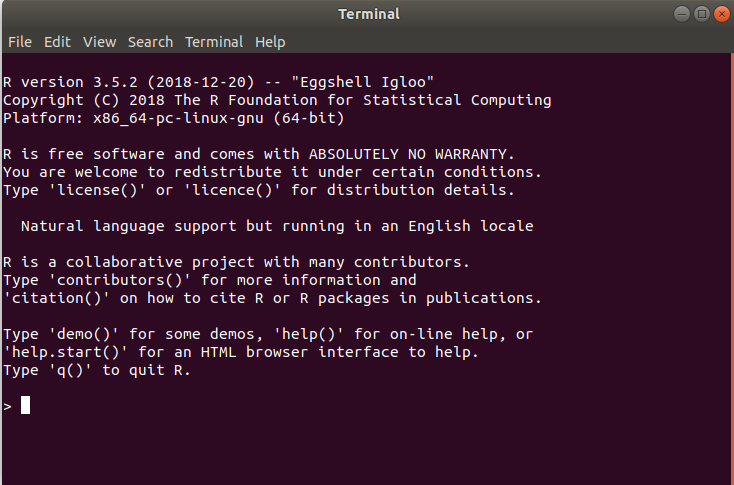
\includegraphics[width=6.02in]{img/R_cmd}

\subsection{Install RStudio}\label{install-rstudio}

To get the most out of R we recommend installing the RStudio
\citep{noauthor_rstudio_2019} integrated development environment. It is
an environment that provides a console with a range of features to
enrich the use of R.

To download, visit \url{https://www.rstudio.com/products/rstudio/} and
follow the instructions for your system.

The end results should look similar to this:

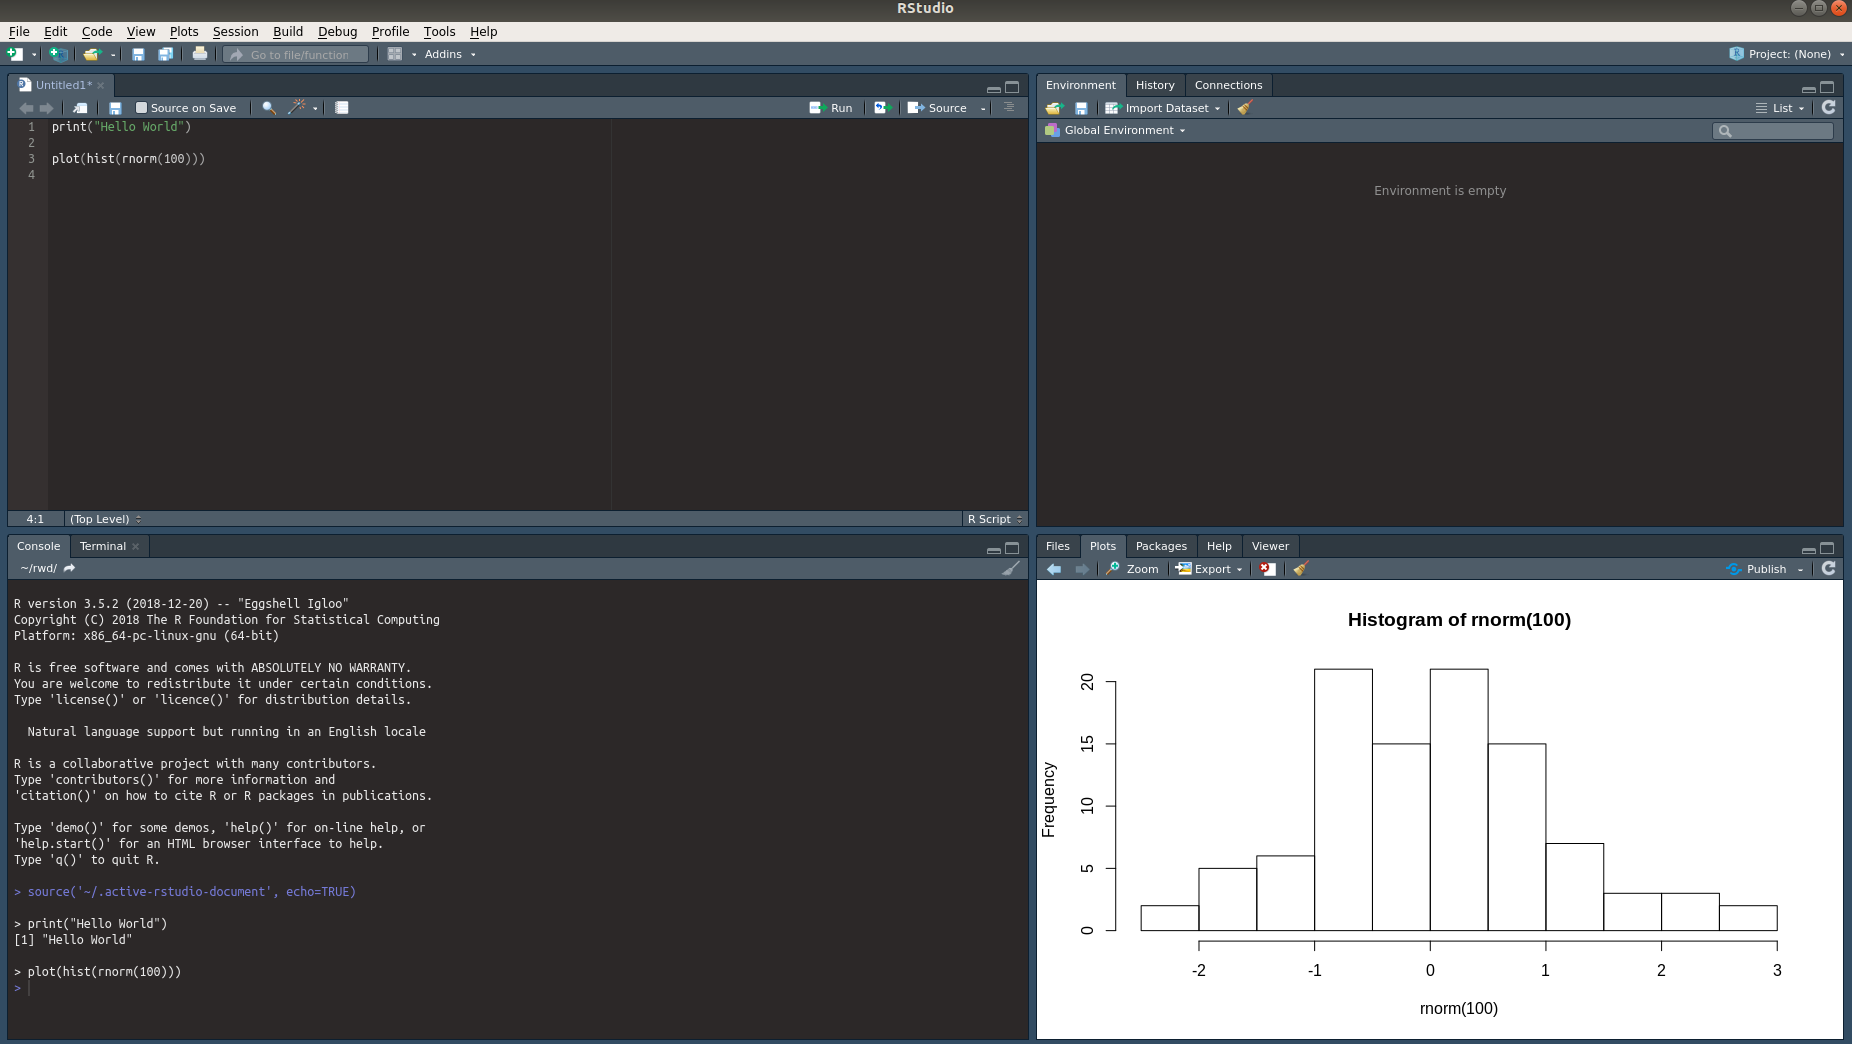
\includegraphics[width=6.01in]{img/rstudio}

\subsection{Install Required R
Packages}\label{install-required-r-packages}

R has a ecosystem of open source packages that work like add-ins. These
packages typically contain specialised functionality that may be
required when performing analysis. You can install R packages from the R
console and they will be downloaded onto your system and available
whenever you use R.

The main R packages we will use in this paper are:

\begin{itemize}
\item
  \href{https://www.tidyverse.org/}{tidyverse} - The tidyverse is an
  opinionated collection of R packages designed for data science. All
  packages share an underlying design philosophy, grammar, and data
  structures. \citep{R-tidyverse}
\item
  \href{https://bigrquery.r-dbi.org/}{bigrquery} - The bigrquery package
  makes it easy to work with data stored in Google BigQuery by allowing
  you to query BigQuery tables and retrieve metadata about your
  projects, data sets, tables, and jobs. \citep{R-bigrquery}
\item
  \href{https://cran.r-project.org/web/packages/ChannelAttribution}{ChannelAttribution}
  - Implements a Markov Model for the Online Multi-Channel Attribution
  Problem. \citep{R-ChannelAttribution}
\item
  \href{https://cran.r-project.org/web/packages/survival/}{survival} -
  Contains the core survival analysis routines, including definition of
  Surv objects, Kaplan-Meier and Aalen-Johansen (multi-state) curves,
  Cox models, and parametric accelerated failure time models.
  \citep{R-survival}
\item
  \href{https://cran.r-project.org/web/packages/CausalImpact/}{CausalImpact}
  - Implements a Bayesian approach to causal impact estimation in time
  series, as described in \citet{causalimpact}
\end{itemize}

To install these packages, and some other supporting packages used in
this paper, you can run the command below

\begin{Shaded}
\begin{Highlighting}[]
\KeywordTok{install.packages}\NormalTok{(}\KeywordTok{c}\NormalTok{(}\StringTok{"tidyverse"}\NormalTok{, }\StringTok{"bigrquery"}\NormalTok{, }\StringTok{"ChannelAttribtion"}\NormalTok{, }\StringTok{"survival"}\NormalTok{,}
                   \StringTok{"lubridate"}\NormalTok{, }\StringTok{"survminer"}\NormalTok{, }\StringTok{"DBI"}\NormalTok{, }\StringTok{"CausalImpact"}\NormalTok{))}
\end{Highlighting}
\end{Shaded}

\section{BigQuery}\label{bigquery-1}

The first step to more advanced modelling is extracting and cleaning the
data. Here we will go through a basic setup and familiarisation guide to
get your Analytics data from BigQuery. It is expected that you have some
experience using SQL and knowledge of basic database operations.

\hypertarget{setup-1}{\subsection{Setup}\label{setup-1}}

If you are an Analytics 360 customer, you can setup BigQuery for use
with Google Analytics data. Refer to the
\href{https://support.google.com/analytics/answer/3416092?hl=en\&ref_topic=3416089}{Google
Help Pages} for detailed instructions.

If you don't yet have Analytics 360, you can still benefit from these
practical code examples by using the free
\href{https://support.google.com/analytics/answer/7586738?hl=en\&ref_topic=3416089}{Google
Analytics Sample Dataset}. This is a complete Google Analytics 360 data
set from the Google Merchant Store, a real eCommerce platform.

To access the data set follow the instructions provided by
\href{https://support.google.com/analytics/answer/7586738?hl=en\&ref_topic=3416089}{Google}:

\begin{enumerate}
\def\labelenumi{\arabic{enumi}.}
\item
  Go to \url{http://bigquery.cloud.google.com}.
\item
  If you're new to BigQuery, or you don't have a project set up yet,
  you'll need to create a project.
\item
  Select this
  \href{https://bigquery.cloud.google.com/table/bigquery-public-data:google_analytics_sample.ga_sessions_20170801?pli=1}{link}
  to go directly to the data set.
\item
  Click \textbf{Query Table} to run a query.
\end{enumerate}

In the future you can access the data set within BigQuery by selecting
the \texttt{bigquery-public-data} project from the left-hand navigation
panel, then select the \texttt{ga\_sessions} table under the
\texttt{google\_analytics\_sample} data set.

Please be mindful that using BigQuery can incur a cost. Please refer to
Google's billing and quota information before use.

\subsection{Export Schema}\label{export-schema}

The way Google Analytics structures its data export into BigQuery is
known as the export schema. This schema is able to take advantage of
data structures that may be counter-intuitive for users who are familiar
with normalised relational databases. BigQuery supports de-normalised
tables, where instead of joining lots of flat, normalised tables, you
can have one table with nested records.

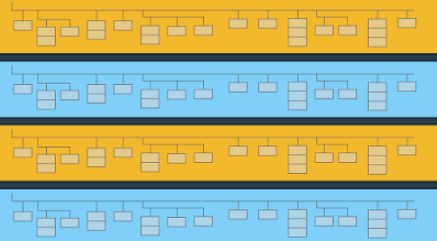
\includegraphics[width=4.37in]{img/bqexport}

In the bigquery data set, there is one table per day, defined at the
session level that contains all Analytics related data nested within,
such as hits and events. Below we will demonstrate some basic queries on
this data.

For more information you can refer to the
\href{https://support.google.com/analytics/answer/3437719?hl=en\&ref_topic=3416089\#}{BigQuery
Export Schema}

\subsection{Running Queries}\label{running-queries}

\subsubsection{Hello World}\label{hello-world}

This is a basic query to run that simply sums the page views over a
given day. You will note the use of \texttt{\#standardSQL} in the
header. This lets bigquery know you are using the `standard' SQL flavour
over it's older `legacy' flavour.

\begin{Shaded}
\begin{Highlighting}[]
\CommentTok{/* Hello World Example */}
\NormalTok{#standardSQL}
\KeywordTok{SELECT} \FunctionTok{SUM}\NormalTok{(totals.pageviews) }\KeywordTok{as}\NormalTok{ TotalPageviews}
    
\KeywordTok{FROM}\NormalTok{ `bigquery-public-data.google_analytics_sample.ga_sessions_20170101`}
\end{Highlighting}
\end{Shaded}

\begin{longtable}[]{@{}ll@{}}
\toprule
Row & TotalPageviews\tabularnewline
\midrule
\endhead
1 & 5362\tabularnewline
\bottomrule
\end{longtable}

\subsubsection{Using Table Ranges}\label{using-table-ranges}

As the GA Export Schema provides one table per day, to scan across date
ranges we need to specify a table range to query.

Notice the \texttt{*} in the FROM clause and the inclusion of
\texttt{\_TABLE\_SUFFIX}.

\begin{Shaded}
\begin{Highlighting}[]
\CommentTok{/* Using Table Ranges */}
\NormalTok{#standardSQL}
\KeywordTok{SELECT}  \DataTypeTok{date}\NormalTok{, }
        \FunctionTok{SUM}\NormalTok{(totals.pageviews) }\KeywordTok{as}\NormalTok{ TotalPageviews}

\KeywordTok{FROM}\NormalTok{  `bigquery-public-data.google_analytics_sample.ga_sessions_*`}

\KeywordTok{WHERE}\NormalTok{ _TABLE_SUFFIX }\KeywordTok{BETWEEN} \StringTok{'20170725'} \KeywordTok{AND} \StringTok{'20170801'}

\KeywordTok{GROUP} \KeywordTok{BY} \DataTypeTok{date}

\KeywordTok{ORDER} \KeywordTok{BY} \DataTypeTok{date}
\end{Highlighting}
\end{Shaded}

\subsubsection{Hit Level Data}\label{hit-level-data}

Accessing `hit' level data, that is, individual hits within each user's
session requires `un-nesting' the hits data and joining it to the
\texttt{ga\_sessions\_} table

\begin{Shaded}
\begin{Highlighting}[]
\CommentTok{/* Now at the hit level */}
\NormalTok{#standardSQL}
\KeywordTok{SELECT}\NormalTok{  fullVisitorId,  }
\NormalTok{        visitNumber, }
        \DataTypeTok{date}\NormalTok{, }
\NormalTok{        totals.hits, }
\NormalTok{        hits.hitNumber, }
\NormalTok{        hits.type, }
\NormalTok{        hits.time, }
\NormalTok{        hits.page.pagePath}
        
\KeywordTok{FROM}\NormalTok{ `bigquery-public-data.google_analytics_sample.ga_sessions_20170101`,}
\NormalTok{  UNNEST(hits) }\KeywordTok{as}\NormalTok{ hits}
  
\KeywordTok{WHERE}\NormalTok{ fullVisitorId = }\StringTok{'6170732910727440668'} \CommentTok{/*Random Visitor Selected*/}
\end{Highlighting}
\end{Shaded}

Now that we are equipped with the basics we can further our
understanding in future chapters to extract the data we need for
modelling.

\hypertarget{using-r-with-bigquery}{\subsection{Using R with
BigQuery}\label{using-r-with-bigquery}}

We can also interact with the BigQuery API using the \texttt{bigrquery}
package in R.

To set up we load this package, along with the \texttt{DBI} package
which helps with database interfacing.

\begin{Shaded}
\begin{Highlighting}[]
\KeywordTok{library}\NormalTok{(bigrquery)}
\KeywordTok{library}\NormalTok{(DBI)}
\end{Highlighting}
\end{Shaded}

Next we establish a connection to BigQuery. Here you would replace
\texttt{bq\_test\_project()} with the project id you have established in
Google Cloud Console.

\begin{Shaded}
\begin{Highlighting}[]
\NormalTok{con <-}\StringTok{ }\KeywordTok{dbConnect}\NormalTok{(}
\NormalTok{  bigrquery}\OperatorTok{::}\KeywordTok{bigquery}\NormalTok{(),}
  \DataTypeTok{project =} \StringTok{"bigquery-public-data"}\NormalTok{,}
  \DataTypeTok{dataset =} \StringTok{"google_analytics_sample"}\NormalTok{,}
  \DataTypeTok{billing =} \KeywordTok{bq_test_project}\NormalTok{()}
\NormalTok{)}
\end{Highlighting}
\end{Shaded}

We can save any SQL queries and forward these for execution as text
strings.

\begin{Shaded}
\begin{Highlighting}[]
\NormalTok{sql <-}\StringTok{ "}
\StringTok{  /* Using Table Ranges */}
\StringTok{  #standardSQL}
\StringTok{  SELECT  date, }
\StringTok{        SUM(totals.pageviews) as TotalPageviews}
\StringTok{  }
\StringTok{  FROM  `bigquery-public-data.google_analytics_sample.ga_sessions_*`}
\StringTok{  }
\StringTok{  WHERE _TABLE_SUFFIX BETWEEN '20170725' AND '20170801'}
\StringTok{  }
\StringTok{  GROUP BY date}
\StringTok{  }
\StringTok{  ORDER BY date}
\StringTok{  "}
\end{Highlighting}
\end{Shaded}

Here the query is executed and saved as a temp table. The
\texttt{bq\_table\_download} function returns the results to the
console.

\begin{Shaded}
\begin{Highlighting}[]
\NormalTok{query <-}\StringTok{ }\KeywordTok{bq_project_query}\NormalTok{(}\DataTypeTok{x =} \KeywordTok{bq_test_project}\NormalTok{(), sql)}
\KeywordTok{bq_table_download}\NormalTok{(query)}
\end{Highlighting}
\end{Shaded}

\begin{tabular}{l|r}
\hline
date & TotalPageviews\\
\hline
20170725 & 10728\\
\hline
20170726 & 11200\\
\hline
20170727 & 10175\\
\hline
20170728 & 9359\\
\hline
20170729 & 6293\\
\hline
20170730 & 7258\\
\hline
20170731 & 11115\\
\hline
20170801 & 10939\\
\hline
\end{tabular}

\chapter{Extracting Data from
BigQuery}\label{extracting-data-from-bigquery}

The first step before we implement our own attribution models in R is to
extract the data from BigQuery. Here we assume you are a Google
Analytics 360 customer and have set up the BiqQuery export. If you are
using some other form of multi-touch conversion pathway data, you can
skip this section. For this example we will be using the
\texttt{bigquery-public-data} data set which contains a sample of
Analytics 360 data from the Google Merchant Store (See
\protect\hyperlink{setup-1}{Section 6.2} for setup info).

\hypertarget{about-the-data}{\section{About the
data}\label{about-the-data}}

When we conduct this analysis, a key consideration is how much data to
use.

It's usually not feasible, or sensible to use all available clickstream
data in your organisation. Here we have made some decisions around how
much data we want to base our models on.

\begin{itemize}
\tightlist
\item
  Extract the last 30 days of sessions\\
\item
  Keep both converting and non-converting users\\
\item
  Look back 7 days of touch points from the visitor's most recent
  session.\\
\item
  If the visitor converted, disregard any subsequent visits.
\end{itemize}

These numbers are arbitrary and should be considered in light of your
organisation. Some websites with a longer conversion funnel may want to
analyse 6 months of data, using a look back window of one month for
example.

\section{Get full event log}\label{get-full-event-log}

First we want to extract a log of all sessions during a time period.
Here we have selected 30 days. Note how we use the \texttt{*} suffix in
the \texttt{FROM} clause so we can scan multiple dates at once.

We have selected the \texttt{fullVisitorId} as the unique identifier. A
time stamp of the \texttt{visitStartTime} and the
\texttt{channelGrouping} which will show the Default Channel Group
associated with an end user's session for this View.

\begin{Shaded}
\begin{Highlighting}[]
   \KeywordTok{SELECT}\NormalTok{ fullVisitorId, }
\NormalTok{          TIMESTAMP_SECONDS(SAFE_CAST(visitStartTime }\KeywordTok{AS}\NormalTok{ INT64))  }\KeywordTok{AS}\NormalTok{ visitStartTime,  }
\NormalTok{          channelGrouping}

    \KeywordTok{FROM}\NormalTok{ `bigquery-public-data.google_analytics_sample.ga_sessions_*`}

    \KeywordTok{WHERE}\NormalTok{ _TABLE_SUFFIX }\KeywordTok{BETWEEN} \StringTok{'20170101'} \KeywordTok{AND} \StringTok{'20170131'}

    \KeywordTok{ORDER} \KeywordTok{BY}\NormalTok{ fullVisitorId, visitStartTime}
\end{Highlighting}
\end{Shaded}

\section{Identify those who
converted}\label{identify-those-who-converted}

Next we identify all visitors who made a transaction during our date
range, and the date of this transaction. We have specified a
`transaction' as our conversion goal, however there is no reason why
this can't be another goal, such as a sign up event etc.

\begin{Shaded}
\begin{Highlighting}[]
    \KeywordTok{SELECT}\NormalTok{ fullVisitorId, }
           \FunctionTok{MIN}\NormalTok{(TIMESTAMP_SECONDS(SAFE_CAST(visitStartTime }\KeywordTok{AS}\NormalTok{ INT64)))  }\KeywordTok{AS}\NormalTok{ purchasetime}

    \KeywordTok{FROM}\NormalTok{ `bigquery-public-data.google_analytics_sample.ga_sessions_*`}

    \KeywordTok{WHERE}\NormalTok{ _TABLE_SUFFIX }\KeywordTok{BETWEEN} \StringTok{'20170101'} \KeywordTok{AND} \StringTok{'20170131'}
     \KeywordTok{AND}\NormalTok{ totals.transactions }\KeywordTok{IS} \KeywordTok{NOT} \KeywordTok{NULL}

    \KeywordTok{GROUP} \KeywordTok{BY}\NormalTok{ fullVisitorId}

    \KeywordTok{ORDER} \KeywordTok{BY}\NormalTok{ fullVisitorId}
\end{Highlighting}
\end{Shaded}

\section{Converting touchpoints in last 7
days}\label{converting-touchpoints-in-last-7-days}

Now we can identify our converting path touch points. These are taken
from the event log we defined in Step 1, however we ensure only visitors
who converted appear in our results. Furthermore we restrict the results
to only those touch points that occur on or before the purchase time
(obviously touch points after this don't influence the conversion
outcome). Finally we implement a look-back period of 7 days, so any
touch points older than this are disregarded.

\begin{Shaded}
\begin{Highlighting}[]
  \KeywordTok{SELECT}\NormalTok{ a.*,}
         \StringTok{'conversion'} \KeywordTok{AS}\NormalTok{ outcome}

  \KeywordTok{FROM}\NormalTok{ event_log a}
    \KeywordTok{INNER} \KeywordTok{JOIN}\NormalTok{ conversions b }\KeywordTok{ON}\NormalTok{ a.fullVisitorId = b.fullVisitorId  }

  \KeywordTok{WHERE}\NormalTok{ a.visitStartTime <= b.purchasetime }
    \KeywordTok{AND}\NormalTok{ DATE_DIFF(}\DataTypeTok{DATE}\NormalTok{(b.purchasetime), }\DataTypeTok{DATE}\NormalTok{(a.visitStartTime), }\DataTypeTok{DAY}\NormalTok{)  <= }\DecValTok{7}
\end{Highlighting}
\end{Shaded}

\section{Non-converting touchpoints in last 7
days}\label{non-converting-touchpoints-in-last-7-days}

For those users who did not convert, we need to identify the most recent
session start time so we can calculate where to start our 7 day look
back period.

\begin{Shaded}
\begin{Highlighting}[]

\KeywordTok{SELECT}\NormalTok{ fullVisitorId, }
  \FunctionTok{MAX}\NormalTok{(visitStartTime) }\KeywordTok{AS}\NormalTok{ maxvisittime}
  
  \KeywordTok{FROM}\NormalTok{ event_log}
  
  \KeywordTok{GROUP} \KeywordTok{BY}\NormalTok{ fullVisitorId}
\end{Highlighting}
\end{Shaded}

Now we can query the touch points of our non-converting visitors and
apply our 7 day time window.

\begin{Shaded}
\begin{Highlighting}[]
\KeywordTok{SELECT}\NormalTok{ a.*,}
         \StringTok{'non_conversion'} \KeywordTok{AS}\NormalTok{ outcome}

  \KeywordTok{FROM}\NormalTok{ event_log a}
    \KeywordTok{INNER} \KeywordTok{JOIN}\NormalTok{ maxtimes b }\KeywordTok{ON}\NormalTok{ a.fullVisitorId = b.fullVisitorId }

  \KeywordTok{WHERE}\NormalTok{ a.fullVisitorId }\KeywordTok{NOT} \KeywordTok{IN}\NormalTok{ (}\KeywordTok{SELECT} \KeywordTok{DISTINCT}\NormalTok{ fullVisitorID }\KeywordTok{FROM}\NormalTok{ conversions)}
   \KeywordTok{AND}\NormalTok{  DATE_DIFF(}\DataTypeTok{DATE}\NormalTok{(b.maxvisittime), }\DataTypeTok{DATE}\NormalTok{(a.visitStartTime), }\DataTypeTok{DAY}\NormalTok{) <= }\DecValTok{7}
\end{Highlighting}
\end{Shaded}

\section{Complete Query}\label{complete-query}

We can bundle this together to run as one query:

\begin{Shaded}
\begin{Highlighting}[]
\NormalTok{#standardSQL}

\KeywordTok{WITH} 
  \CommentTok{/* EVENT LOG */}
\NormalTok{  event_log }\KeywordTok{AS}\NormalTok{ (}
    \KeywordTok{SELECT}\NormalTok{ fullVisitorId, }
\NormalTok{          TIMESTAMP_SECONDS(SAFE_CAST(visitStartTime }\KeywordTok{AS}\NormalTok{ INT64))  }\KeywordTok{AS}\NormalTok{ visitStartTime,  }
\NormalTok{          channelGrouping}

    \KeywordTok{FROM}\NormalTok{ `bigquery-public-data.google_analytics_sample.ga_sessions_*`}

    \KeywordTok{WHERE}\NormalTok{ _TABLE_SUFFIX }\KeywordTok{BETWEEN} \StringTok{'20170101'} \KeywordTok{AND} \StringTok{'20170131'}

    \KeywordTok{ORDER} \KeywordTok{BY}\NormalTok{ fullVisitorId, visitStartTime}
\NormalTok{  ),}

 \CommentTok{/* VISITORS WHO CONVERTED */}
\NormalTok{ conversions }\KeywordTok{AS}\NormalTok{ (}
    \KeywordTok{SELECT}\NormalTok{ fullVisitorId, }
           \FunctionTok{MIN}\NormalTok{(TIMESTAMP_SECONDS(SAFE_CAST(visitStartTime }\KeywordTok{AS}\NormalTok{ INT64)))  }\KeywordTok{AS}\NormalTok{ purchasetime}

    \KeywordTok{FROM}\NormalTok{ `bigquery-public-data.google_analytics_sample.ga_sessions_*`}

    \KeywordTok{WHERE}\NormalTok{ _TABLE_SUFFIX }\KeywordTok{BETWEEN} \StringTok{'20170101'} \KeywordTok{AND} \StringTok{'20170131'}
     \KeywordTok{AND}\NormalTok{ totals.transactions }\KeywordTok{IS} \KeywordTok{NOT} \KeywordTok{NULL}

    \KeywordTok{GROUP} \KeywordTok{BY}\NormalTok{ fullVisitorId}

    \KeywordTok{ORDER} \KeywordTok{BY}\NormalTok{ fullVisitorId}
\NormalTok{  ),}
  
  \CommentTok{/* LATEST VISIT TIME FOR ALL VISITORS */}
\NormalTok{   maxtimes }\KeywordTok{AS}\NormalTok{ (}
    \KeywordTok{SELECT}\NormalTok{ fullVisitorId, }
    \FunctionTok{MAX}\NormalTok{(visitStartTime) }\KeywordTok{AS}\NormalTok{ maxvisittime}
    
    \KeywordTok{FROM}\NormalTok{ event_log}
    
    \KeywordTok{GROUP} \KeywordTok{BY}\NormalTok{ fullVisitorId}
\NormalTok{  )}

  \CommentTok{/*== MAIN QUERY THAT UNIONS CONVERTING AND NON CONVERTING PATHS WITHA GIVEN TIME WINDOW ==*/}
  
  \CommentTok{/* CONVERTING PATHS */}
  \KeywordTok{SELECT}\NormalTok{ a.*,}
         \StringTok{'conversion'} \KeywordTok{AS}\NormalTok{ outcome}

  \KeywordTok{FROM}\NormalTok{ event_log a}
    \KeywordTok{INNER} \KeywordTok{JOIN}\NormalTok{ conversions b }\KeywordTok{ON}\NormalTok{ a.fullVisitorId = b.fullVisitorId  }

  \KeywordTok{WHERE}\NormalTok{ a.visitStartTime <= b.purchasetime }
    \KeywordTok{AND}\NormalTok{ DATE_DIFF(}\DataTypeTok{DATE}\NormalTok{(b.purchasetime), }\DataTypeTok{DATE}\NormalTok{(a.visitStartTime), }\DataTypeTok{DAY}\NormalTok{)  <= }\DecValTok{7}

\KeywordTok{UNION} \KeywordTok{ALL}

  \CommentTok{/* NON CONVERTING PATHS */}
  \KeywordTok{SELECT}\NormalTok{ a.*,}
         \StringTok{'non_conversion'} \KeywordTok{AS}\NormalTok{ outcome}

  \KeywordTok{FROM}\NormalTok{ event_log a}
    \KeywordTok{INNER} \KeywordTok{JOIN}\NormalTok{ maxtimes b }\KeywordTok{ON}\NormalTok{ a.fullVisitorId = b.fullVisitorId }

  \KeywordTok{WHERE}\NormalTok{ a.fullVisitorId }\KeywordTok{NOT} \KeywordTok{IN}\NormalTok{ (}\KeywordTok{SELECT} \KeywordTok{DISTINCT}\NormalTok{ fullVisitorID }\KeywordTok{FROM}\NormalTok{ conversions)}
   \KeywordTok{AND}\NormalTok{  DATE_DIFF(}\DataTypeTok{DATE}\NormalTok{(b.maxvisittime), }\DataTypeTok{DATE}\NormalTok{(a.visitStartTime), }\DataTypeTok{DAY}\NormalTok{) <= }\DecValTok{7}
\end{Highlighting}
\end{Shaded}

\chapter{Heuristic Models}\label{heuristic-models}

Here we will implement some non-algorithmic methods as a baseline. To do
this we will use the
\href{https://cran.r-project.org/web/packages/ChannelAttribution}{ChannelAttribution
R package}

\hypertarget{transform-data}{\section{Transform
Data}\label{transform-data}}

The \texttt{ChannelAttribution} package requires the data structured in
a certain way. In this case it is in the form:

\begin{longtable}[]{@{}lll@{}}
\toprule
path & conversion & non-conversions\tabularnewline
\midrule
\endhead
direct \textgreater{} social \textgreater{} search & 10 &
154\tabularnewline
direct \textgreater{} direct \textgreater{} direct & 2 &
234\tabularnewline
referral \textgreater{} direct & 7 & 187\tabularnewline
\bottomrule
\end{longtable}

Here the touch points are transformed from into a single string path,
separated by the \texttt{\textgreater{}} character. For each path we
aggregate the total number of conversions that resulted from this
pathway, and also the number of non-conversions.

If you are using marketing data from a system other than BigQuery, you
will need to prepare your data per the above.

Now we can look at the steps required to transform our data from
\protect\hyperlink{about-the-data}{Chapter 7}.

In this case we have the results saved as a CSV, but these may also be
queried directly in R as per
\protect\hyperlink{using-r-with-bigquery}{Section 6.2.4}

\begin{Shaded}
\begin{Highlighting}[]
\KeywordTok{library}\NormalTok{(tidyverse)}
\KeywordTok{library}\NormalTok{(lubridate)}

\NormalTok{paths_raw <-}\StringTok{ }\KeywordTok{read_csv}\NormalTok{(}\StringTok{'bigquery/bq-results.csv'}\NormalTok{)}
\end{Highlighting}
\end{Shaded}

Below is a snapshot of the top 20 rows. We can see from BigQuery it is
in a standard `long' format with one row per touch point based on the
time stamp.

\begin{tabular}{l|l|l|l}
\hline
fullVisitorId & visitStartTime & channelGrouping & outcome\\
\hline
07184911138250312 & 2017-01-18 06:57:50 UTC & (Other) & non\_conversion\\
\hline
07184911138250312 & 2017-01-18 07:40:31 UTC & (Other) & non\_conversion\\
\hline
07184911138250312 & 2017-01-18 08:18:50 UTC & (Other) & non\_conversion\\
\hline
3112985461863519829 & 2017-01-25 20:42:23 UTC & (Other) & non\_conversion\\
\hline
4720404071621394560 & 2017-01-18 07:02:40 UTC & (Other) & non\_conversion\\
\hline
6060076679741207514 & 2017-01-18 06:59:27 UTC & (Other) & non\_conversion\\
\hline
0003297619580760716 & 2017-01-08 05:50:50 UTC & Direct & non\_conversion\\
\hline
00035794135966385 & 2017-01-20 12:46:25 UTC & Direct & non\_conversion\\
\hline
0004867638405459898 & 2017-01-15 14:22:26 UTC & Direct & non\_conversion\\
\hline
0005604256236421547 & 2017-01-24 21:04:26 UTC & Direct & non\_conversion\\
\hline
0006746295360194683 & 2017-01-24 05:16:18 UTC & Direct & non\_conversion\\
\hline
0009834325573666752 & 2017-01-24 22:43:34 UTC & Direct & non\_conversion\\
\hline
001324382917654255 & 2017-01-10 18:46:32 UTC & Direct & non\_conversion\\
\hline
0013701781325366363 & 2017-01-25 15:32:52 UTC & Direct & non\_conversion\\
\hline
0014256672578655164 & 2017-01-24 17:39:56 UTC & Direct & non\_conversion\\
\hline
0015731153666510386 & 2017-01-25 22:37:42 UTC & Direct & non\_conversion\\
\hline
0016316356325418630 & 2017-01-09 03:08:40 UTC & Direct & non\_conversion\\
\hline
0016883628233932470 & 2017-01-04 18:02:46 UTC & Direct & non\_conversion\\
\hline
0017373815580187343 & 2017-01-25 11:59:15 UTC & Direct & non\_conversion\\
\hline
0018094491063949293 & 2017-01-18 15:18:19 UTC & Direct & non\_conversion\\
\hline
\end{tabular}

We are using the \texttt{tidyverse} conventions here to make the
interpretation easier. To translate we can see we start by formatting
the time stamp correctly.\\
Next we rank the sessions by this time stamp for each visitor so we know
which order the touch points occurred. We next restructure the data by
summarising the touch points into one path string. Finally we count the
occurrence of conversions and non-conversions.

\begin{Shaded}
\begin{Highlighting}[]
\NormalTok{paths <-}\StringTok{ }\NormalTok{paths_raw }\OperatorTok\StringTok{ }
\StringTok{  }\KeywordTok{mutate}\NormalTok{(}\DataTypeTok{visitStartTime =} \KeywordTok{ymd_hms}\NormalTok{(visitStartTime)) }\OperatorTok\StringTok{ }
\StringTok{  }\KeywordTok{group_by}\NormalTok{(fullVisitorId, outcome) }\OperatorTok\StringTok{ }
\StringTok{  }\KeywordTok{arrange}\NormalTok{(visitStartTime) }\OperatorTok\StringTok{ }
\StringTok{  }\KeywordTok{summarise}\NormalTok{(}\DataTypeTok{path =} \KeywordTok{paste}\NormalTok{(channelGrouping, }\DataTypeTok{collapse =} \StringTok{' > '}\NormalTok{)) }\OperatorTok\StringTok{ }
\StringTok{  }\KeywordTok{ungroup}\NormalTok{() }\OperatorTok\StringTok{ }
\StringTok{  }\KeywordTok{count}\NormalTok{(outcome, path, }\DataTypeTok{name =} \StringTok{"n"}\NormalTok{) }\OperatorTok\StringTok{ }
\StringTok{  }\KeywordTok{spread}\NormalTok{(outcome, n) }\OperatorTok\StringTok{ }
\StringTok{  }\KeywordTok{replace_na}\NormalTok{(}\KeywordTok{list}\NormalTok{(}\DataTypeTok{conversion =} \DecValTok{0}\NormalTok{, }\DataTypeTok{non_conversion =} \DecValTok{0}\NormalTok{)) }\OperatorTok\StringTok{ }
\StringTok{  }\KeywordTok{arrange}\NormalTok{(}\KeywordTok{desc}\NormalTok{(conversion))}
\end{Highlighting}
\end{Shaded}

\begin{tabular}{l|r|r}
\hline
path & conversion & non\_conversion\\
\hline
Referral & 178 & 4015\\
\hline
Organic Search & 137 & 21659\\
\hline
Direct & 71 & 9308\\
\hline
Referral > Referral & 55 & 553\\
\hline
Organic Search > Organic Search & 39 & 1507\\
\hline
Direct > Direct & 26 & 803\\
\hline
Referral > Referral > Referral & 26 & 132\\
\hline
Paid Search & 21 & 1348\\
\hline
Display & 12 & 256\\
\hline
Direct > Referral & 11 & 60\\
\hline
\end{tabular}

\section{Heuristic Models}\label{heuristic-models-1}

Now that the data are in the correct format we can use the
\texttt{ChannelAttribution::heuristic\_models()} function to compare
three common models: First Touch, Last Touch and Linear.

This function will automatically calculate the total number of
conversion attributed to each channel using the above models.

The results across these three methods are very similar. We can see
`Referral' is the channel that is attributed the most credit for
conversions, followed by `Organic Search'.

The Last Touch method provides slightly more credit to `Referral' than
other methods, in contrast to `Direct', which is attributed more credit
when using the First Touch method.

\begin{Shaded}
\begin{Highlighting}[]
\KeywordTok{library}\NormalTok{(ChannelAttribution)}

\NormalTok{fit_h <-}\StringTok{ }\KeywordTok{heuristic_models}\NormalTok{(}\DataTypeTok{Data =}\NormalTok{ paths, }\DataTypeTok{var_path =} \StringTok{'path'}\NormalTok{, }\DataTypeTok{var_conv =} \StringTok{'conversion'}\NormalTok{)}
\end{Highlighting}
\end{Shaded}

\begin{tabular}{l|r|r|r}
\hline
channel\_name & first\_touch & last\_touch & linear\_touch\\
\hline
Referral & 279 & 302 & 290.46667\\
\hline
Organic Search & 203 & 202 & 202.28333\\
\hline
Direct & 124 & 106 & 114.31667\\
\hline
Paid Search & 31 & 26 & 29.08333\\
\hline
Display & 19 & 20 & 19.85000\\
\hline
Social & 6 & 6 & 6.00000\\
\hline
(Other) & 0 & 0 & 0.00000\\
\hline
Affiliates & 0 & 0 & 0.00000\\
\hline
\end{tabular}

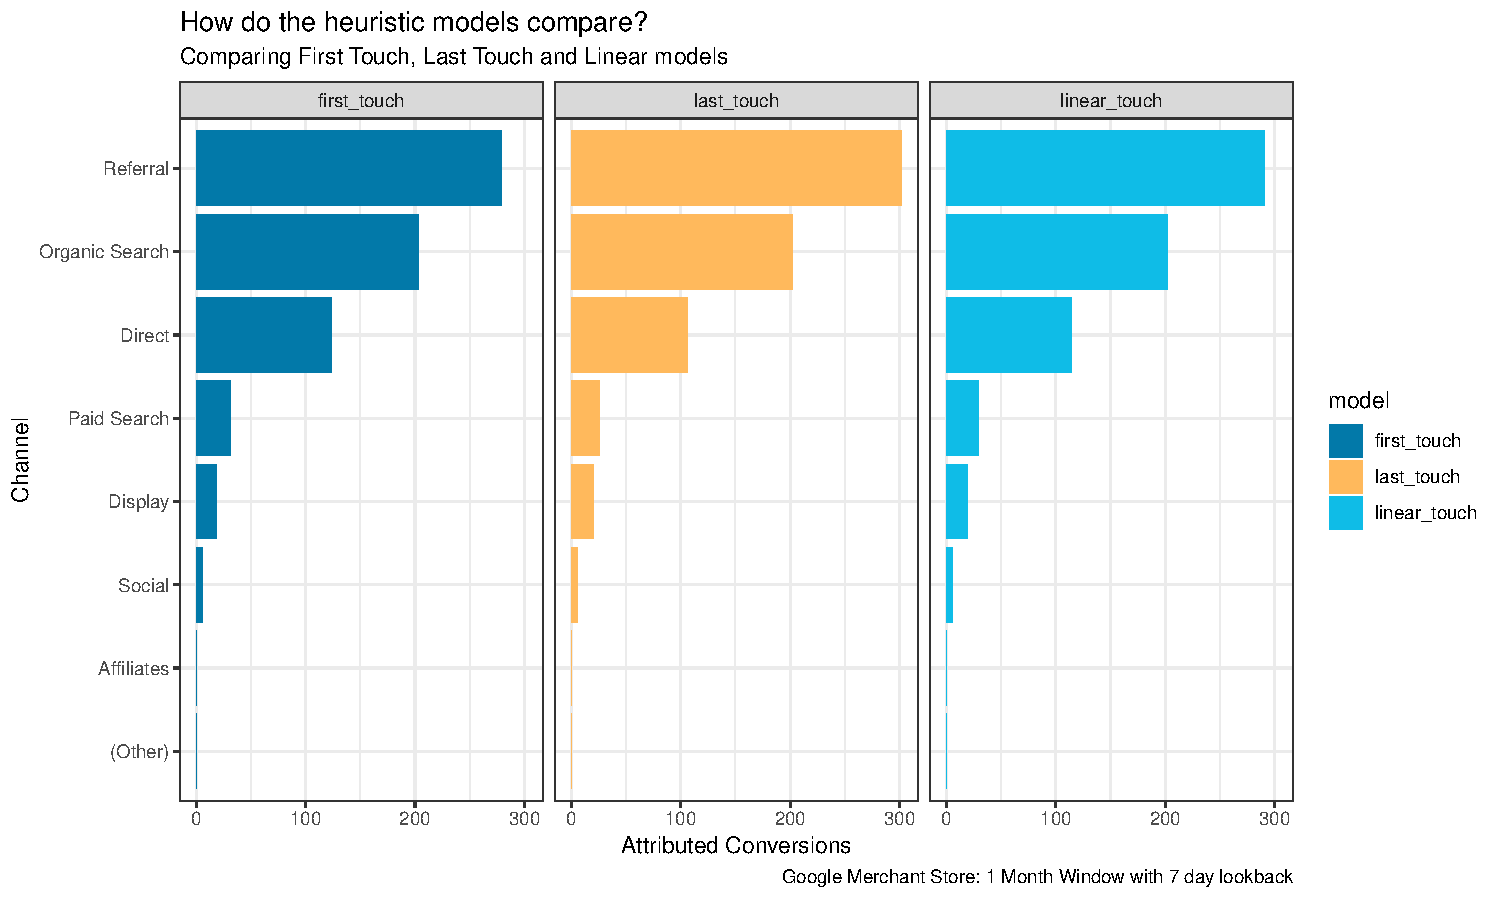
\includegraphics{irx-attribution-2019_files/figure-latex/unnamed-chunk-49-1.pdf}

\chapter{Algorithmic Methods}\label{algorithmic-methods}

Now we move into algorithmic methods for modelling marketing
attribution.

These methods use more advanced statistical algorithms to create a data
driven model for assigning conversion credit to channels in a
multi-touch point conversion pathway.

\hypertarget{markov-chains}{\section{Markov
Chains}\label{markov-chains}}

The first method we will review are markov chains. We introduced these
in \protect\hyperlink{markov-methods}{section 4.3.3}.

First we load the required packages. In this case we again use
\texttt{ChannelAttribution} as well as the \texttt{tidyverse} and
\texttt{lubridate} packages for data manipulation and date handling. We
also read in our raw results from BigQuery that contains the event log
and timestamps of visits, complete with channel and outcome.

\begin{Shaded}
\begin{Highlighting}[]
\KeywordTok{library}\NormalTok{(tidyverse)}
\KeywordTok{library}\NormalTok{(lubridate)}
\KeywordTok{library}\NormalTok{(ChannelAttribution)}

\NormalTok{paths_raw <-}\StringTok{ }\KeywordTok{read_csv}\NormalTok{(}\StringTok{'bigquery/bq-results.csv'}\NormalTok{)}
\end{Highlighting}
\end{Shaded}

\begin{tabular}{l|l|l|l}
\hline
fullVisitorId & visitStartTime & channelGrouping & outcome\\
\hline
07184911138250312 & 2017-01-18 06:57:50 UTC & (Other) & non\_conversion\\
\hline
07184911138250312 & 2017-01-18 07:40:31 UTC & (Other) & non\_conversion\\
\hline
07184911138250312 & 2017-01-18 08:18:50 UTC & (Other) & non\_conversion\\
\hline
3112985461863519829 & 2017-01-25 20:42:23 UTC & (Other) & non\_conversion\\
\hline
4720404071621394560 & 2017-01-18 07:02:40 UTC & (Other) & non\_conversion\\
\hline
6060076679741207514 & 2017-01-18 06:59:27 UTC & (Other) & non\_conversion\\
\hline
0003297619580760716 & 2017-01-08 05:50:50 UTC & Direct & non\_conversion\\
\hline
00035794135966385 & 2017-01-20 12:46:25 UTC & Direct & non\_conversion\\
\hline
0004867638405459898 & 2017-01-15 14:22:26 UTC & Direct & non\_conversion\\
\hline
0005604256236421547 & 2017-01-24 21:04:26 UTC & Direct & non\_conversion\\
\hline
\end{tabular}

Next we need to transform the data. We use the same procedure as in
\protect\hyperlink{transform-data}{Section 7.1}. We now have one row per
conversion path, with total conversions/non-conversions.

\begin{tabular}{l|r|r}
\hline
path & conversion & non\_conversion\\
\hline
Referral & 178 & 4015\\
\hline
Organic Search & 137 & 21659\\
\hline
Direct & 71 & 9308\\
\hline
Referral > Referral & 55 & 553\\
\hline
Organic Search > Organic Search & 39 & 1507\\
\hline
Direct > Direct & 26 & 803\\
\hline
Referral > Referral > Referral & 26 & 132\\
\hline
Paid Search & 21 & 1348\\
\hline
Display & 12 & 256\\
\hline
Direct > Referral & 11 & 60\\
\hline
\end{tabular}

We now call the \texttt{markov\_model()} function from the
\texttt{ChannelAttribution} package. It accepts arguments for the data
frame, the variable that contains the conversion path, the variable that
encodes both number of conversions and non conversions and the order of
the markov model.

Below we can see it's output is a list of distinct channels with the
total attributed conversions per channel. The channel that receives the
most credit is `Referral', followed by `Organic Search'.

As a marketer we could multiply these by the average conversion value to
get a total attributed value for each channel. By comparing this to the
cost of marketing in each channel we get a robust calculation for ROI.

In fact, if the actual sales revenue per customer is recorded we can go
one step further and have this model calculate the attributed value
without having to estimate using the average value. This is handled with
the argument \texttt{var\_value}.

\begin{Shaded}
\begin{Highlighting}[]
\NormalTok{fit_m <-}\StringTok{ }\KeywordTok{markov_model}\NormalTok{(}\DataTypeTok{Data =}\NormalTok{ paths, }
                      \DataTypeTok{var_path =} \StringTok{'path'}\NormalTok{, }
                      \DataTypeTok{var_conv =} \StringTok{'conversion'}\NormalTok{, }
                      \DataTypeTok{var_null =} \StringTok{'non_conversion'}\NormalTok{, }
                      \DataTypeTok{order =} \DecValTok{1}\NormalTok{)}

\NormalTok{fit_m}
\end{Highlighting}
\end{Shaded}

\begin{verbatim}
##     channel_name total_conversions
## 1       Referral       289.7406085
## 2 Organic Search       209.9964297
## 3         Direct       106.2056815
## 4    Paid Search        27.3863707
## 5        Display        19.7819000
## 6         Social         7.2961813
## 7        (Other)         0.1541447
## 8     Affiliates         1.4386836
\end{verbatim}

We can also iterate on this by calculating a 1, 2, and 3 order markov
model.

Below we display a chart of the results. As we can see, there is not
much difference in the results.

\begin{Shaded}
\begin{Highlighting}[]
\NormalTok{fit_mult <-}\StringTok{ }\KeywordTok{map_dfr}\NormalTok{(}\DataTypeTok{.x =} \KeywordTok{c}\NormalTok{(}\DecValTok{1}\NormalTok{, }\DecValTok{2}\NormalTok{, }\DecValTok{3}\NormalTok{), }
                    \DataTypeTok{.f =} \OperatorTok{~}\KeywordTok{markov_model}\NormalTok{(}\DataTypeTok{Data =}\NormalTok{ paths, }
                                       \DataTypeTok{var_path =} \StringTok{'path'}\NormalTok{, }
                                       \DataTypeTok{var_conv =} \StringTok{'conversion'}\NormalTok{, }
                                       \DataTypeTok{var_null =} \StringTok{'non_conversion'}\NormalTok{, }
                                       \DataTypeTok{order =}\NormalTok{ .x), }
                    \DataTypeTok{.id =} \StringTok{"order"}\NormalTok{)}
\end{Highlighting}
\end{Shaded}

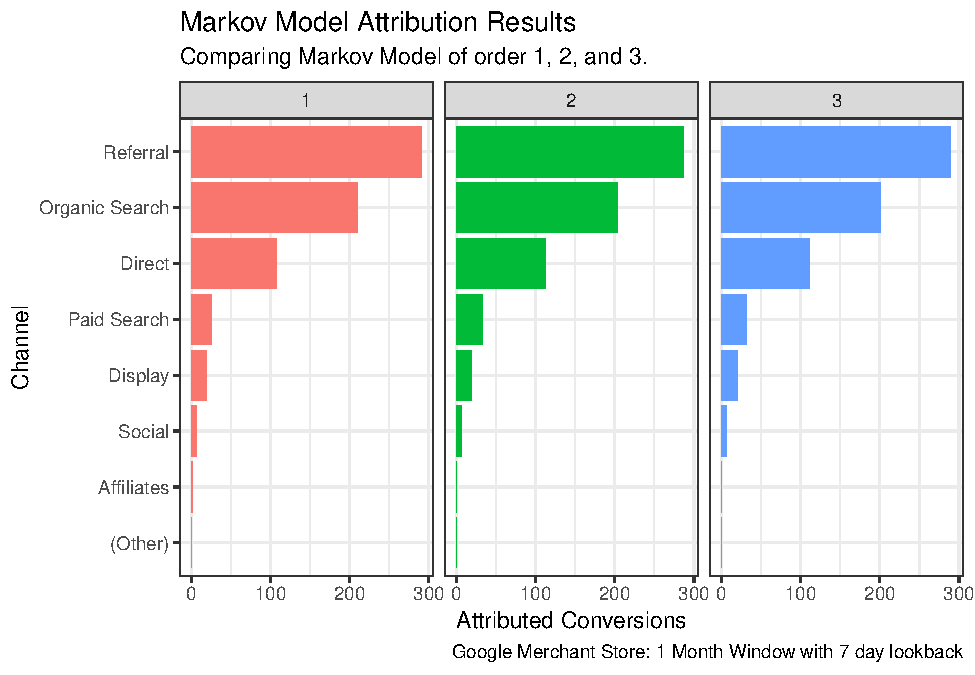
\includegraphics{irx-attribution-2019_files/figure-latex/unnamed-chunk-57-1.pdf}

\hypertarget{survival-analysis}{\section{Survival
Analysis}\label{survival-analysis}}

The next model we demonstrate is survival analysis. Here we define
`survival' as non-conversion and the event of interest is when a
customer converts.

As usual we start by loading the data and the required packages.

\begin{Shaded}
\begin{Highlighting}[]
\KeywordTok{library}\NormalTok{(tidyverse)}
\KeywordTok{library}\NormalTok{(lubridate)}
\KeywordTok{library}\NormalTok{(survival)}
\KeywordTok{library}\NormalTok{(survminer)}

\NormalTok{paths_raw <-}\StringTok{ }\KeywordTok{read_csv}\NormalTok{(}\StringTok{'bigquery/bq-results.csv'}\NormalTok{)}
\end{Highlighting}
\end{Shaded}

\begin{tabular}{l|l|l|l}
\hline
fullVisitorId & visitStartTime & channelGrouping & outcome\\
\hline
07184911138250312 & 2017-01-18 06:57:50 UTC & (Other) & non\_conversion\\
\hline
07184911138250312 & 2017-01-18 07:40:31 UTC & (Other) & non\_conversion\\
\hline
07184911138250312 & 2017-01-18 08:18:50 UTC & (Other) & non\_conversion\\
\hline
3112985461863519829 & 2017-01-25 20:42:23 UTC & (Other) & non\_conversion\\
\hline
4720404071621394560 & 2017-01-18 07:02:40 UTC & (Other) & non\_conversion\\
\hline
6060076679741207514 & 2017-01-18 06:59:27 UTC & (Other) & non\_conversion\\
\hline
0003297619580760716 & 2017-01-08 05:50:50 UTC & Direct & non\_conversion\\
\hline
00035794135966385 & 2017-01-20 12:46:25 UTC & Direct & non\_conversion\\
\hline
0004867638405459898 & 2017-01-15 14:22:26 UTC & Direct & non\_conversion\\
\hline
0005604256236421547 & 2017-01-24 21:04:26 UTC & Direct & non\_conversion\\
\hline
\end{tabular}

The data transformation steps here are a little different.

We want to condense our data into one row per customer. For our
analysis, three key pieces of information are required:

\begin{enumerate}
\def\labelenumi{\arabic{enumi})}
\tightlist
\item
  The interval of time:
\end{enumerate}

\begin{enumerate}
\def\labelenumi{\alph{enumi})}
\tightlist
\item
  For converting customers, between the first visit and the purchase
  time.
\item
  For non-converting customers, between the first visit and the last
  recorded visit.
\end{enumerate}

\begin{enumerate}
\def\labelenumi{\arabic{enumi})}
\setcounter{enumi}{1}
\tightlist
\item
  The outcome: 1 for converted, 0 for non-converted.
\item
  The channel used to convert.
\end{enumerate}

Firstly, this analysis is slightly different. We aren't strictly
attributing credit between channels, but rather analysing at various
points in time, what is the probability of a customer converting through
any given channel.

Secondly, we have made some assumptions around excluding (or censoring)
customers who don't convert at the point of the most recent visit. In
effect we are declaring these customer lost to follow up. An alternative
method would be to calculate the time interval for non-converters right
up until the end of the analysis period. Both are ok, but given we
constrained our look back period to just 7 days we will go with our
chosen method.

\begin{Shaded}
\begin{Highlighting}[]
\NormalTok{surv_data <-}\StringTok{ }\NormalTok{paths_raw }\OperatorTok\StringTok{ }
\StringTok{  }\KeywordTok{mutate}\NormalTok{(}\DataTypeTok{visitStartTime =} \KeywordTok{ymd_hms}\NormalTok{(visitStartTime)) }\OperatorTok\StringTok{ }
\StringTok{  }\KeywordTok{group_by}\NormalTok{(fullVisitorId) }\OperatorTok\StringTok{ }
\StringTok{  }\KeywordTok{mutate}\NormalTok{(}\DataTypeTok{mindate =} \KeywordTok{min}\NormalTok{(visitStartTime),}
         \DataTypeTok{maxdate =} \KeywordTok{max}\NormalTok{(visitStartTime)) }\OperatorTok\StringTok{ }
\StringTok{  }\KeywordTok{filter}\NormalTok{(visitStartTime }\OperatorTok{==}\StringTok{ }\NormalTok{maxdate) }\OperatorTok\StringTok{ }
\StringTok{  }\KeywordTok{mutate}\NormalTok{(}\DataTypeTok{time =}\NormalTok{ (maxdate }\OperatorTok{-}\StringTok{ }\NormalTok{mindate)}\OperatorTok{/}\DecValTok{3600}\NormalTok{,}
         \DataTypeTok{status =} \KeywordTok{ifelse}\NormalTok{(outcome }\OperatorTok{==}\StringTok{ "conversion"}\NormalTok{, }\DecValTok{1}\NormalTok{, }\DecValTok{0}\NormalTok{)) }\OperatorTok\StringTok{ }
\StringTok{  }\NormalTok{dplyr}\OperatorTok{::}\KeywordTok{select}\NormalTok{(fullVisitorId, time, status, channelGrouping)}
\end{Highlighting}
\end{Shaded}

\begin{verbatim}
## # A tibble: 10 x 4
## # Groups:   fullVisitorId [10]
##    fullVisitorId      time        status channelGrouping
##    <chr>              <time>       <dbl> <chr>          
##  1 48853089148264994~ 0.00000000~      0 Social         
##  2 77424453797616436~ 0.00000000~      0 Organic Search 
##  3 35382961118733745~ 0.00000000~      0 Direct         
##  4 22905878572329286~ 0.00000000~      0 Organic Search 
##  5 49866419995749112~ 0.00000000~      0 Organic Search 
##  6 853089376150635567 0.00000000~      0 Organic Search 
##  7 81055338799633676~ 0.00000000~      0 Referral       
##  8 55543663053734243~ 0.00000000~      0 Referral       
##  9 44838988143636314~ 0.01555556~      0 Social         
## 10 836224165758780524 0.00000000~      0 Social
\end{verbatim}

Next we create a special object called a survival object using the
\texttt{Surv} function.

\begin{Shaded}
\begin{Highlighting}[]
\NormalTok{surv_object <-}\StringTok{ }\KeywordTok{Surv}\NormalTok{(}\DataTypeTok{time =}\NormalTok{ surv_data}\OperatorTok{$}\NormalTok{time, }\DataTypeTok{event =}\NormalTok{ surv_data}\OperatorTok{$}\NormalTok{status)}
\end{Highlighting}
\end{Shaded}

We can now compute our estimate for a survival curve using the
\texttt{survfit} function.

We include a grouping variable of the converting channel. This will
calculate one survival curve per group so we have a basis for
comparison.

\begin{Shaded}
\begin{Highlighting}[]
\NormalTok{fit_surv <-}\StringTok{ }\KeywordTok{survfit}\NormalTok{(surv_object }\OperatorTok{~}\StringTok{ }\NormalTok{channelGrouping, }\DataTypeTok{data =}\NormalTok{ surv_data)}
\end{Highlighting}
\end{Shaded}

\begin{verbatim}
## Call: survfit(formula = surv_object ~ channelGrouping, data = surv_data)
## 
##                                    n events median
## channelGrouping=(Other)            2      0     NA
## channelGrouping=Affiliates       963      0     NA
## channelGrouping=Direct         10555    106     NA
## channelGrouping=Display          408     20     NA
## channelGrouping=Organic Search 24208    202     NA
## channelGrouping=Paid Search     1769     26     NA
## channelGrouping=Referral        5372    302     NA
## channelGrouping=Social          9764      6     NA
##                                0.95LCL 0.95UCL
## channelGrouping=(Other)             NA      NA
## channelGrouping=Affiliates          NA      NA
## channelGrouping=Direct             181      NA
## channelGrouping=Display             NA      NA
## channelGrouping=Organic Search      NA      NA
## channelGrouping=Paid Search         NA      NA
## channelGrouping=Referral           174      NA
## channelGrouping=Social              NA      NA
\end{verbatim}

The results are best viewed graphically.

It is important to note that the terminology `survival' in this context
means `non-conversion'. It shows, up to a given time along the x-axis,
what is the probability of a customer \emph{not} converting through a
particular channel.

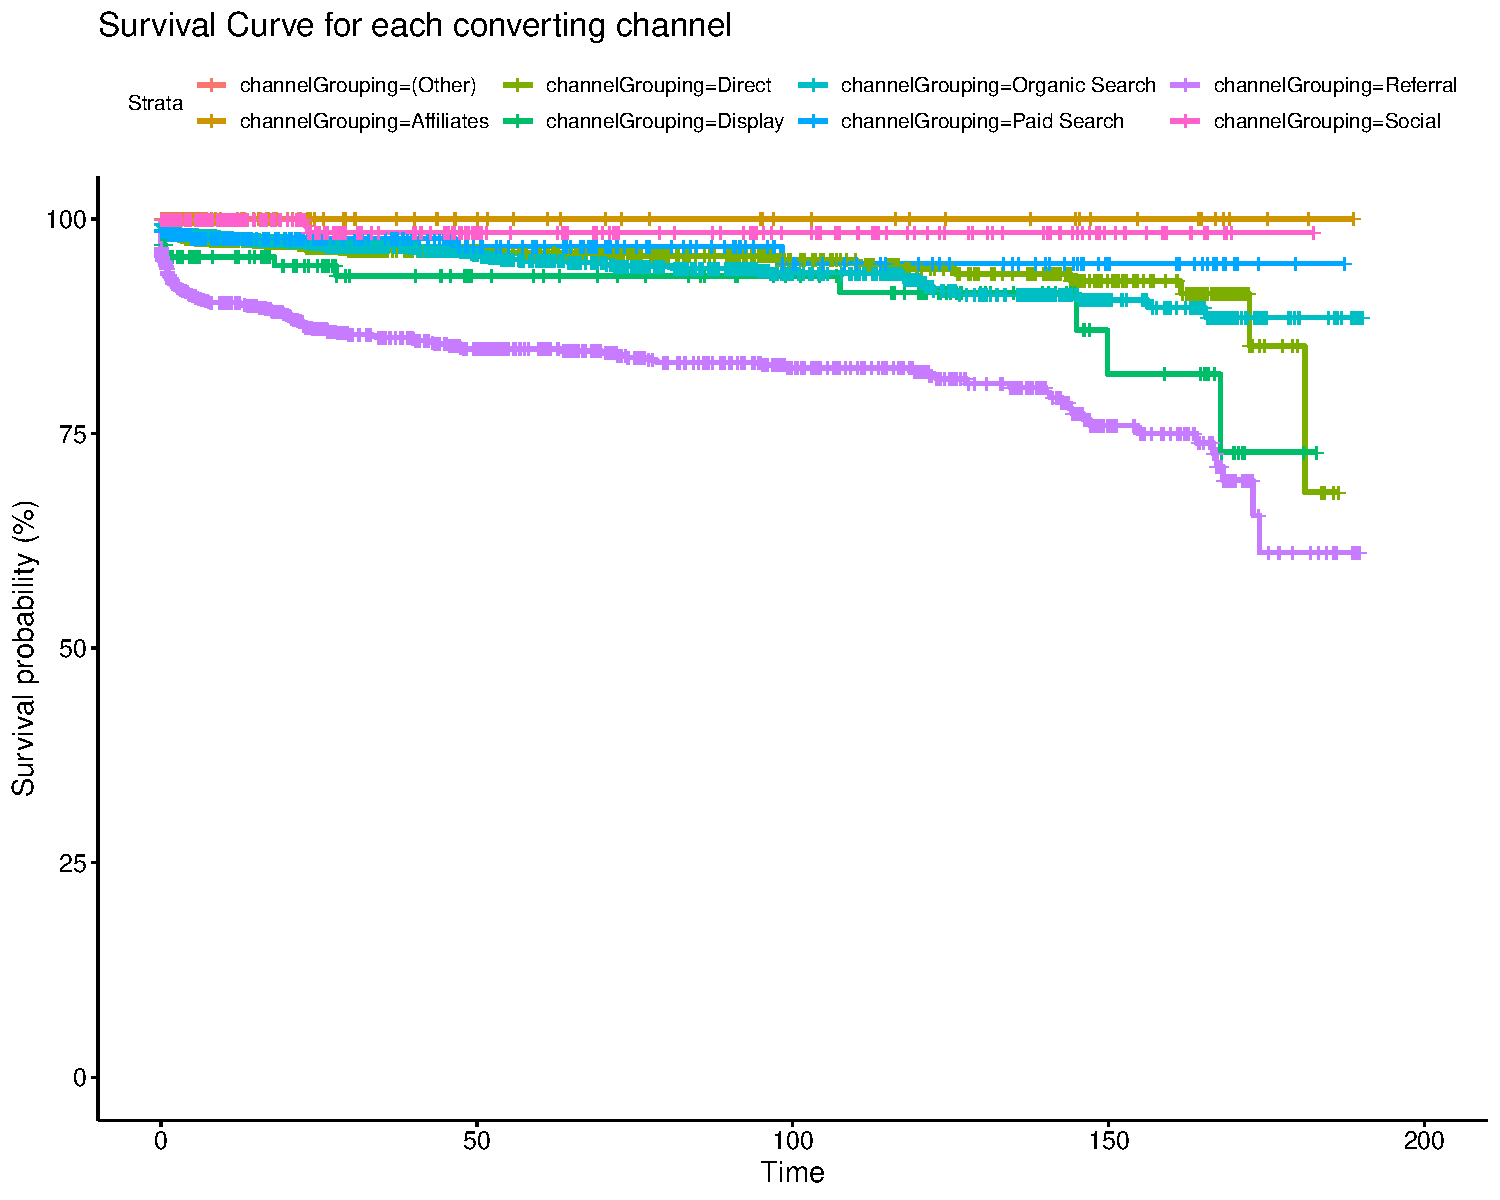
\includegraphics{irx-attribution-2019_files/figure-latex/unnamed-chunk-65-1.pdf}

What we want is the complement of this, that is, the cumulative event
plot.

We can see that Referral channel achieves high levels of conversion very
quickly, representing a valuable channel. This is followed by Display,
however as time goes on, after 150 hours (\textasciitilde{}6 days) from
first visit, channels such as `Direct' and `Organic Search' have a
strong conversion probability. This indicates that advertising and
referral traffic are essential to raising awareness early on, and after
this, customer recall of the brand is high with customers returning days
later via direct and organic channels.

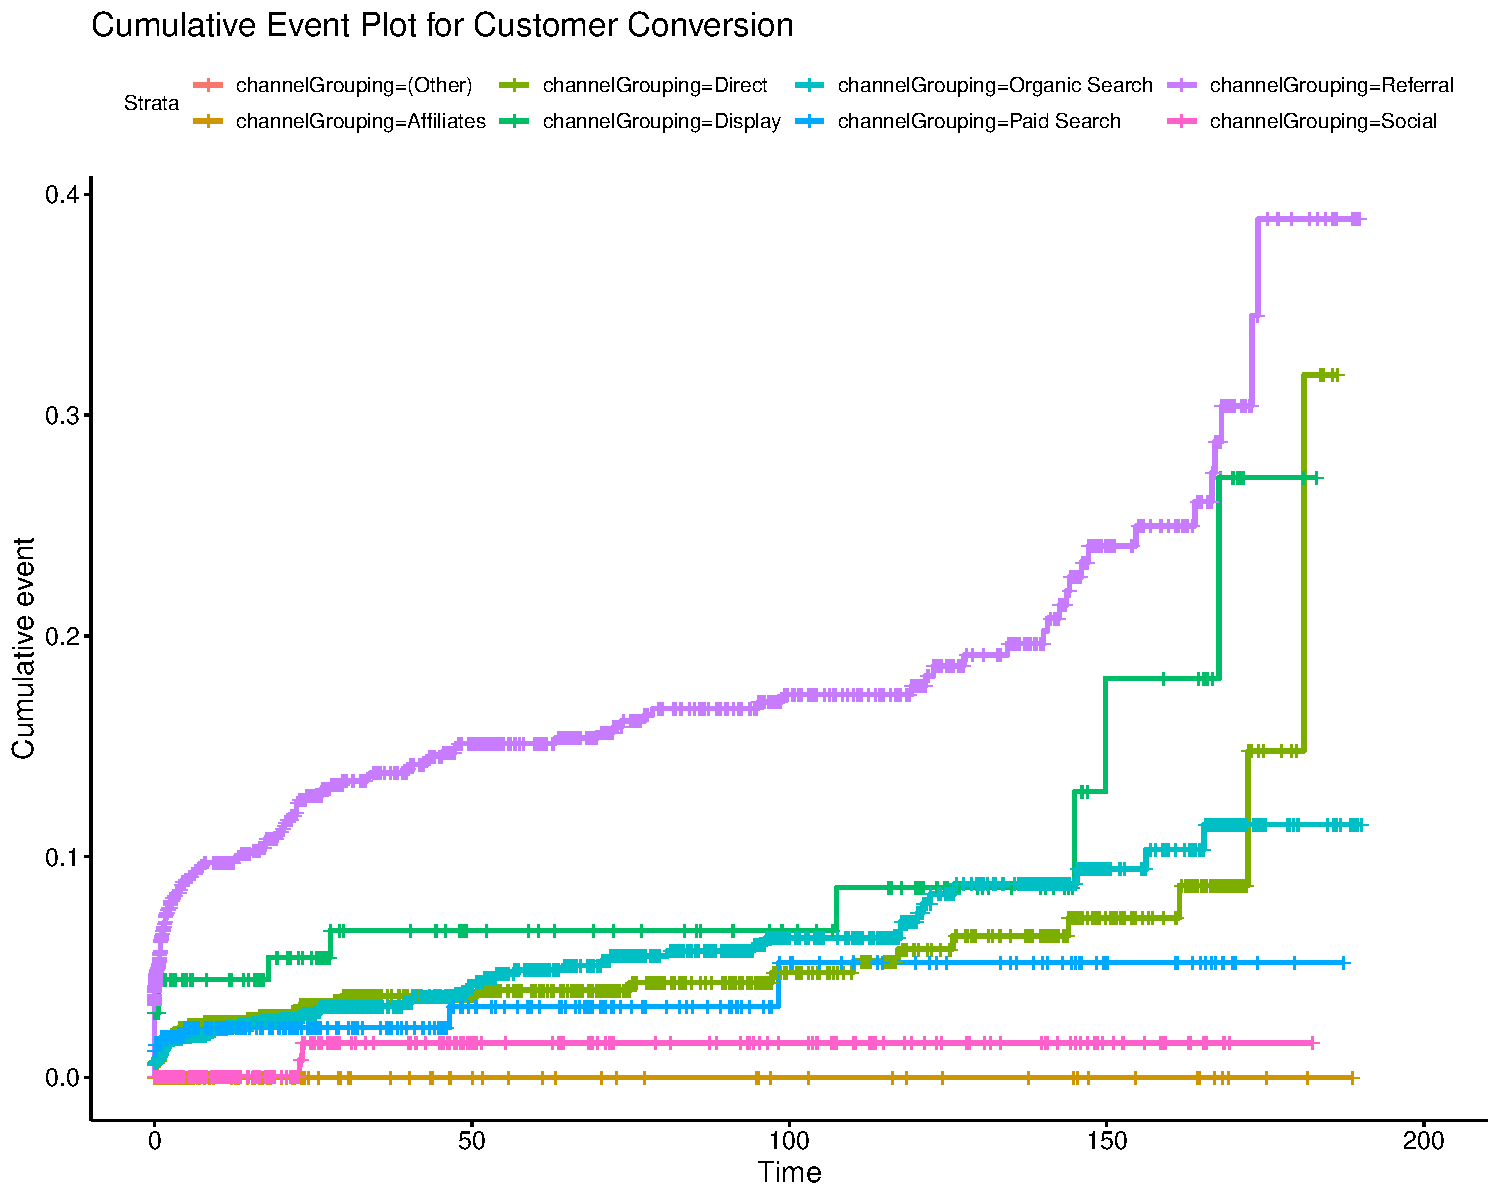
\includegraphics{irx-attribution-2019_files/figure-latex/unnamed-chunk-66-1.pdf}

\part{Offline Attribution}\label{part-offline-attribution}

\chapter{About Offline Attribution}\label{about-offline-attribution}

So far we have looked exclusively at digital marketing. However offline
media channels also play an important part for many businesses.
Generally speaking, the offline media channels include TV, broadcast,
newspaper, coupons and outdoor advertising etc. Compared to online
attribution, it is more difficult to measure the impact of offline
marketing interventions.

When a randomised controlled experiment is not possible, an inferential
method can assist. Below we demonstrate one such method for causal
inference.

Developed by Google, the \texttt{CausalImpact} R package implements
methods for causal inference using Bayesian structural time-series
models \citep{causalimpact}.

Lets see how this works.

\section{Scenario}\label{scenario}

\emph{You run a business that sells widgets. Throughout the year your
product demand and website traffic goes up and down based on a variety
of seasonal factors.\\
You decide to run a TV commercial to promote your product coming into a
busy time of year. This advertisement kicks off on a specified launch
date and runs in just one of your markets (not all regions).}

How can we measure the impact of this TV advertisement on website
traffic?

The intuitive answer is measure the change in sessions before and after
the launch date of the commercial. If we want to get more sophisticated
we might try to compare the change in our advertising region vs.~all
others.

However, a key problem here is recognising what would have happened if
we \textbf{didn't} run our TV commercial. If we timed our campaign to
coincide with a busy time of year, how much of our uplift is due to the
advertising versus just organic uplift? Are we giving the advertising
channel too much credit and inflating our ROI estimates?

\section{Causal Inference Modelling}\label{causal-inference-modelling}

The solution uses a three step process:

\begin{enumerate}
\def\labelenumi{\arabic{enumi})}
\tightlist
\item
  Identify a \emph{control group} which in that case could be website
  sessions from another unaffected region.
\item
  Using historical data from our advertising region, construct a model
  that predicts what would have happened in our advertising region
  during the campaign period if no action was taken. This is called the
  \emph{counterfactual}.
\item
  Compare this counterfactural prediction with the actual number of
  website sessions to calculate the actual uplift attributable to our TV
  commercial.
\end{enumerate}

It is important that the control group selected is not impacted by the
campaign in any way, otherwise the results may be misleading.

Lets first load the packages required:

\begin{Shaded}
\begin{Highlighting}[]
\KeywordTok{library}\NormalTok{(CausalImpact)}
\KeywordTok{library}\NormalTok{(tidyverse)}
\end{Highlighting}
\end{Shaded}

For this example we will simulate some time series data.

The red dashed line is the web traffic for our control region. The solid
black line is the web traffic for our region where the TV commercial is
airing.

We will select our TV campaign period to be from day 70 - 100 with an
uplift of 10 sessions per day.

\begin{Shaded}
\begin{Highlighting}[]
\KeywordTok{set.seed}\NormalTok{(}\DecValTok{2018}\NormalTok{)}
\NormalTok{x1 <-}\StringTok{ }\DecValTok{100} \OperatorTok{+}\StringTok{ }\KeywordTok{arima.sim}\NormalTok{(}\DataTypeTok{model =} \KeywordTok{list}\NormalTok{(}\DataTypeTok{order =} \KeywordTok{c}\NormalTok{(}\DecValTok{1}\NormalTok{,}\DecValTok{1}\NormalTok{,}\DecValTok{0}\NormalTok{), }\DataTypeTok{ar =} \FloatTok{0.7}\NormalTok{), }\DataTypeTok{n =} \DecValTok{99}\NormalTok{)}
\NormalTok{y <-}\StringTok{ }\FloatTok{1.2} \OperatorTok{*}\StringTok{ }\NormalTok{x1 }\OperatorTok{+}\StringTok{ }\KeywordTok{rnorm}\NormalTok{(}\DecValTok{100}\NormalTok{)}
\NormalTok{y[}\DecValTok{70}\OperatorTok{:}\DecValTok{100}\NormalTok{] <-}\StringTok{ }\NormalTok{y[}\DecValTok{70}\OperatorTok{:}\DecValTok{100}\NormalTok{] }\OperatorTok{+}\StringTok{ }\DecValTok{10}
\NormalTok{data <-}\StringTok{ }\KeywordTok{cbind}\NormalTok{(y, x1)}

\KeywordTok{matplot}\NormalTok{(data, }\DataTypeTok{type =} \StringTok{"l"}\NormalTok{)}
\end{Highlighting}
\end{Shaded}

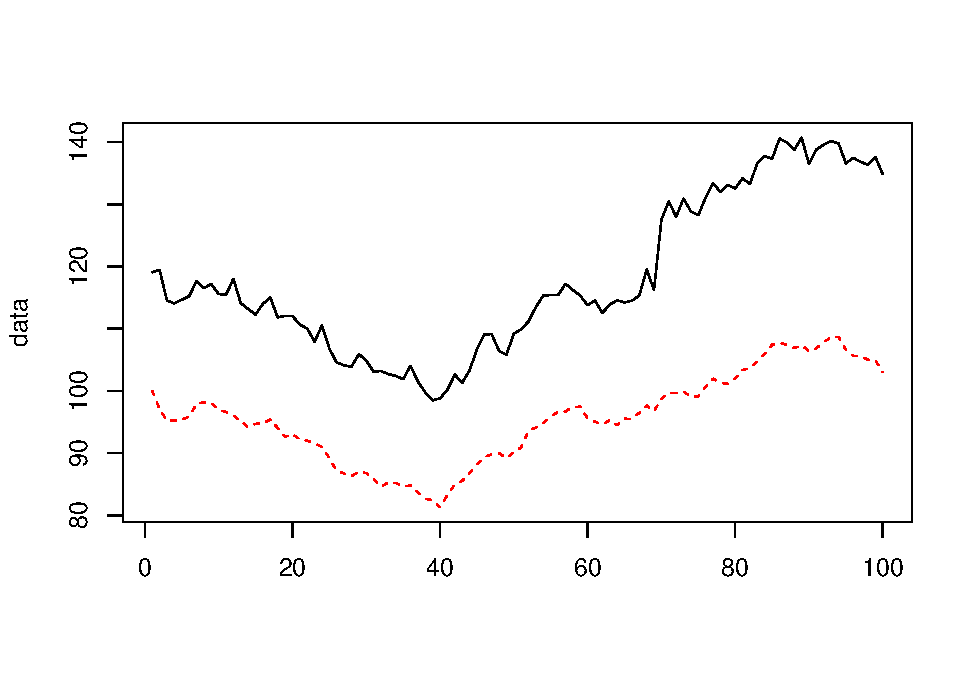
\includegraphics{irx-attribution-2019_files/figure-latex/unnamed-chunk-69-1.pdf}

\begin{Shaded}
\begin{Highlighting}[]
\NormalTok{pre.period <-}\StringTok{ }\KeywordTok{c}\NormalTok{(}\DecValTok{1}\NormalTok{, }\DecValTok{70}\NormalTok{)}
\NormalTok{post.period <-}\StringTok{ }\KeywordTok{c}\NormalTok{(}\DecValTok{71}\NormalTok{, }\DecValTok{100}\NormalTok{)}
\end{Highlighting}
\end{Shaded}

We can now fit the causal inference model using the
\texttt{CausalImpact()} function.

\begin{Shaded}
\begin{Highlighting}[]
\NormalTok{impact <-}\StringTok{ }\KeywordTok{CausalImpact}\NormalTok{(data, pre.period, post.period)}
\end{Highlighting}
\end{Shaded}

\begin{verbatim}
## Posterior inference {CausalImpact}
## 
##                          Average        Cumulative   
## Actual                   135            4062         
## Prediction (s.d.)        125 (0.89)     3765 (26.64) 
## 95% CI                   [124, 127]     [3712, 3817] 
##                                                      
## Absolute effect (s.d.)   9.9 (0.89)     297.2 (26.64)
## 95% CI                   [8.2, 12]      [245.0, 350] 
##                                                      
## Relative effect (s.d.)   7.9% (0.71%)   7.9% (0.71%) 
## 95% CI                   [6.5%, 9.3%]   [6.5%, 9.3%] 
## 
## Posterior tail-area probability p:   0.001
## Posterior prob. of a causal effect:  99.8997%
## 
## For more details, type: summary(impact, "report")
\end{verbatim}

We can also view the results graphically.

The `original' facet shows the actual website visits in the black solid
line and predicted values without marketing intervention in the blue
dashed line. The period of intervention is shown as vertical dashed
lines. The confidence intervals is shaded in blue.

The second, `pointwise' graph basically shows the difference between the
actual values and the predicted values.

The third, `cumulative' graph shows the summed effect of the marketing
intervention after accumulating the differences caused by the marketing
activity since the start date of the intervention.

\begin{Shaded}
\begin{Highlighting}[]
\KeywordTok{plot}\NormalTok{(impact)}
\end{Highlighting}
\end{Shaded}

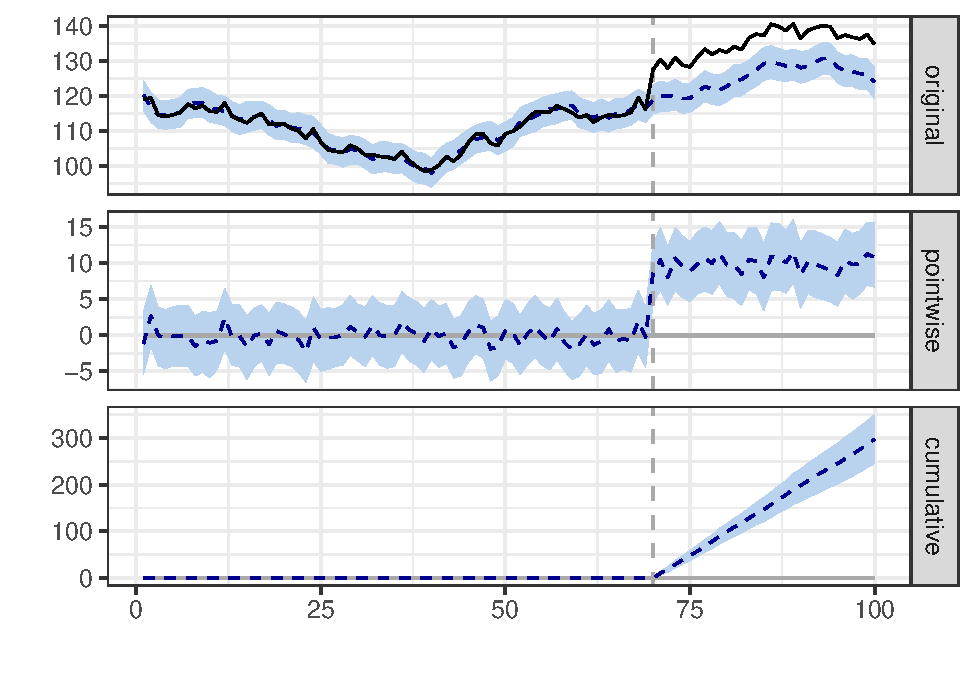
\includegraphics{irx-attribution-2019_files/figure-latex/unnamed-chunk-72-1.pdf}

We can see that the modelled counterfactual increases in the campaign
period, so too does the actual website sessions. Rather than rely on
prior period comparisons we are able to extract the pointwise and
cumulative uplift in a more reasoned way.

We can also generate a written analysis report. We can see the estimate
effect size is 9.91 extra sessions per day, very close to the +10 we
injected in our made-up example.

\begin{Shaded}
\begin{Highlighting}[]
\KeywordTok{summary}\NormalTok{(impact, }\StringTok{"report"}\NormalTok{)}
\end{Highlighting}
\end{Shaded}

\begin{verbatim}
## Analysis report {CausalImpact}
## 
## 
## During the post-intervention period, the response variable had an average value of approx. 135.40. By contrast, in the absence of an intervention, we would have expected an average response of 125.49. The 95% interval of this counterfactual prediction is [123.73, 127.23]. Subtracting this prediction from the observed response yields an estimate of the causal effect the intervention had on the response variable. This effect is 9.91 with a 95% interval of [8.17, 11.66]. For a discussion of the significance of this effect, see below.
## 
## Summing up the individual data points during the post-intervention period (which can only sometimes be meaningfully interpreted), the response variable had an overall value of 4.06K. By contrast, had the intervention not taken place, we would have expected a sum of 3.76K. The 95% interval of this prediction is [3.71K, 3.82K].
## 
## The above results are given in terms of absolute numbers. In relative terms, the response variable showed an increase of +8%. The 95% interval of this percentage is [+7%, +9%].
## 
## This means that the positive effect observed during the intervention period is statistically significant and unlikely to be due to random fluctuations. It should be noted, however, that the question of whether this increase also bears substantive significance can only be answered by comparing the absolute effect (9.91) to the original goal of the underlying intervention.
## 
## The probability of obtaining this effect by chance is very small (Bayesian one-sided tail-area probability p = 0.001). This means the causal effect can be considered statistically significant.
\end{verbatim}

\section{Comparing to other methods}\label{comparing-to-other-methods}

If we rely on a simple, more naive method in this case, we can
overestimate the impact of our TV commercial.

By comparing the average daily web sessions before vs.~after the
campaign started we see an uplift near +25 visits per day. We know this
is an over-estimation as we only injected an uplift of +10 when we
created the synthetic data.

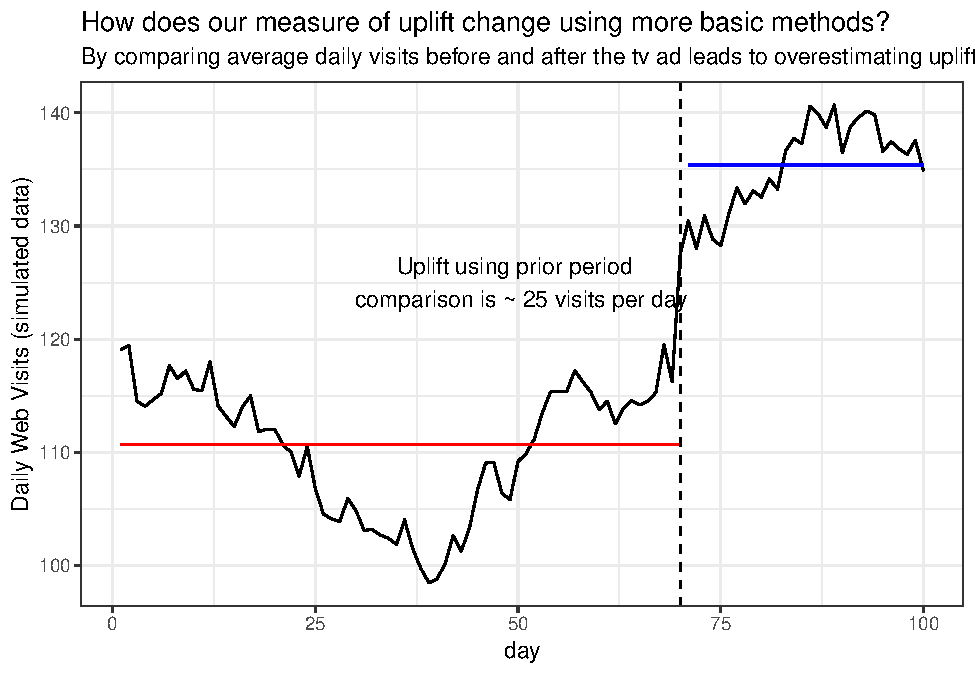
\includegraphics{irx-attribution-2019_files/figure-latex/unnamed-chunk-74-1.pdf}

\bibliography{book.bib,packages.bib}


\end{document}
